\documentclass{article}

\usepackage{graphicx}
\usepackage{hyperref}
\graphicspath{ {./images/} }
\title{
  \huge
  \textbf{Buku Panduan Proxmox}
  \\
  \huge
  Instalasi Pada Server
}

\author{
  \textsc{Classroom Dev Team}
}

\begin{document}
  \pagenumbering{gobble}
  \maketitle

  \newpage
  \pagenumbering{roman}

  \newpage
  \pagenumbering{arabic}
  \section{Proses Instalasi}
  \subsection{Download ISO}
  ISO Proxmox dapat didownload melalui wesite resmi proxmox. \url{https://www.proxmox.com/en/downloads}
  dibawah ini merupakan website proxmox.
  \begin{figure}[h!]
    \centering
    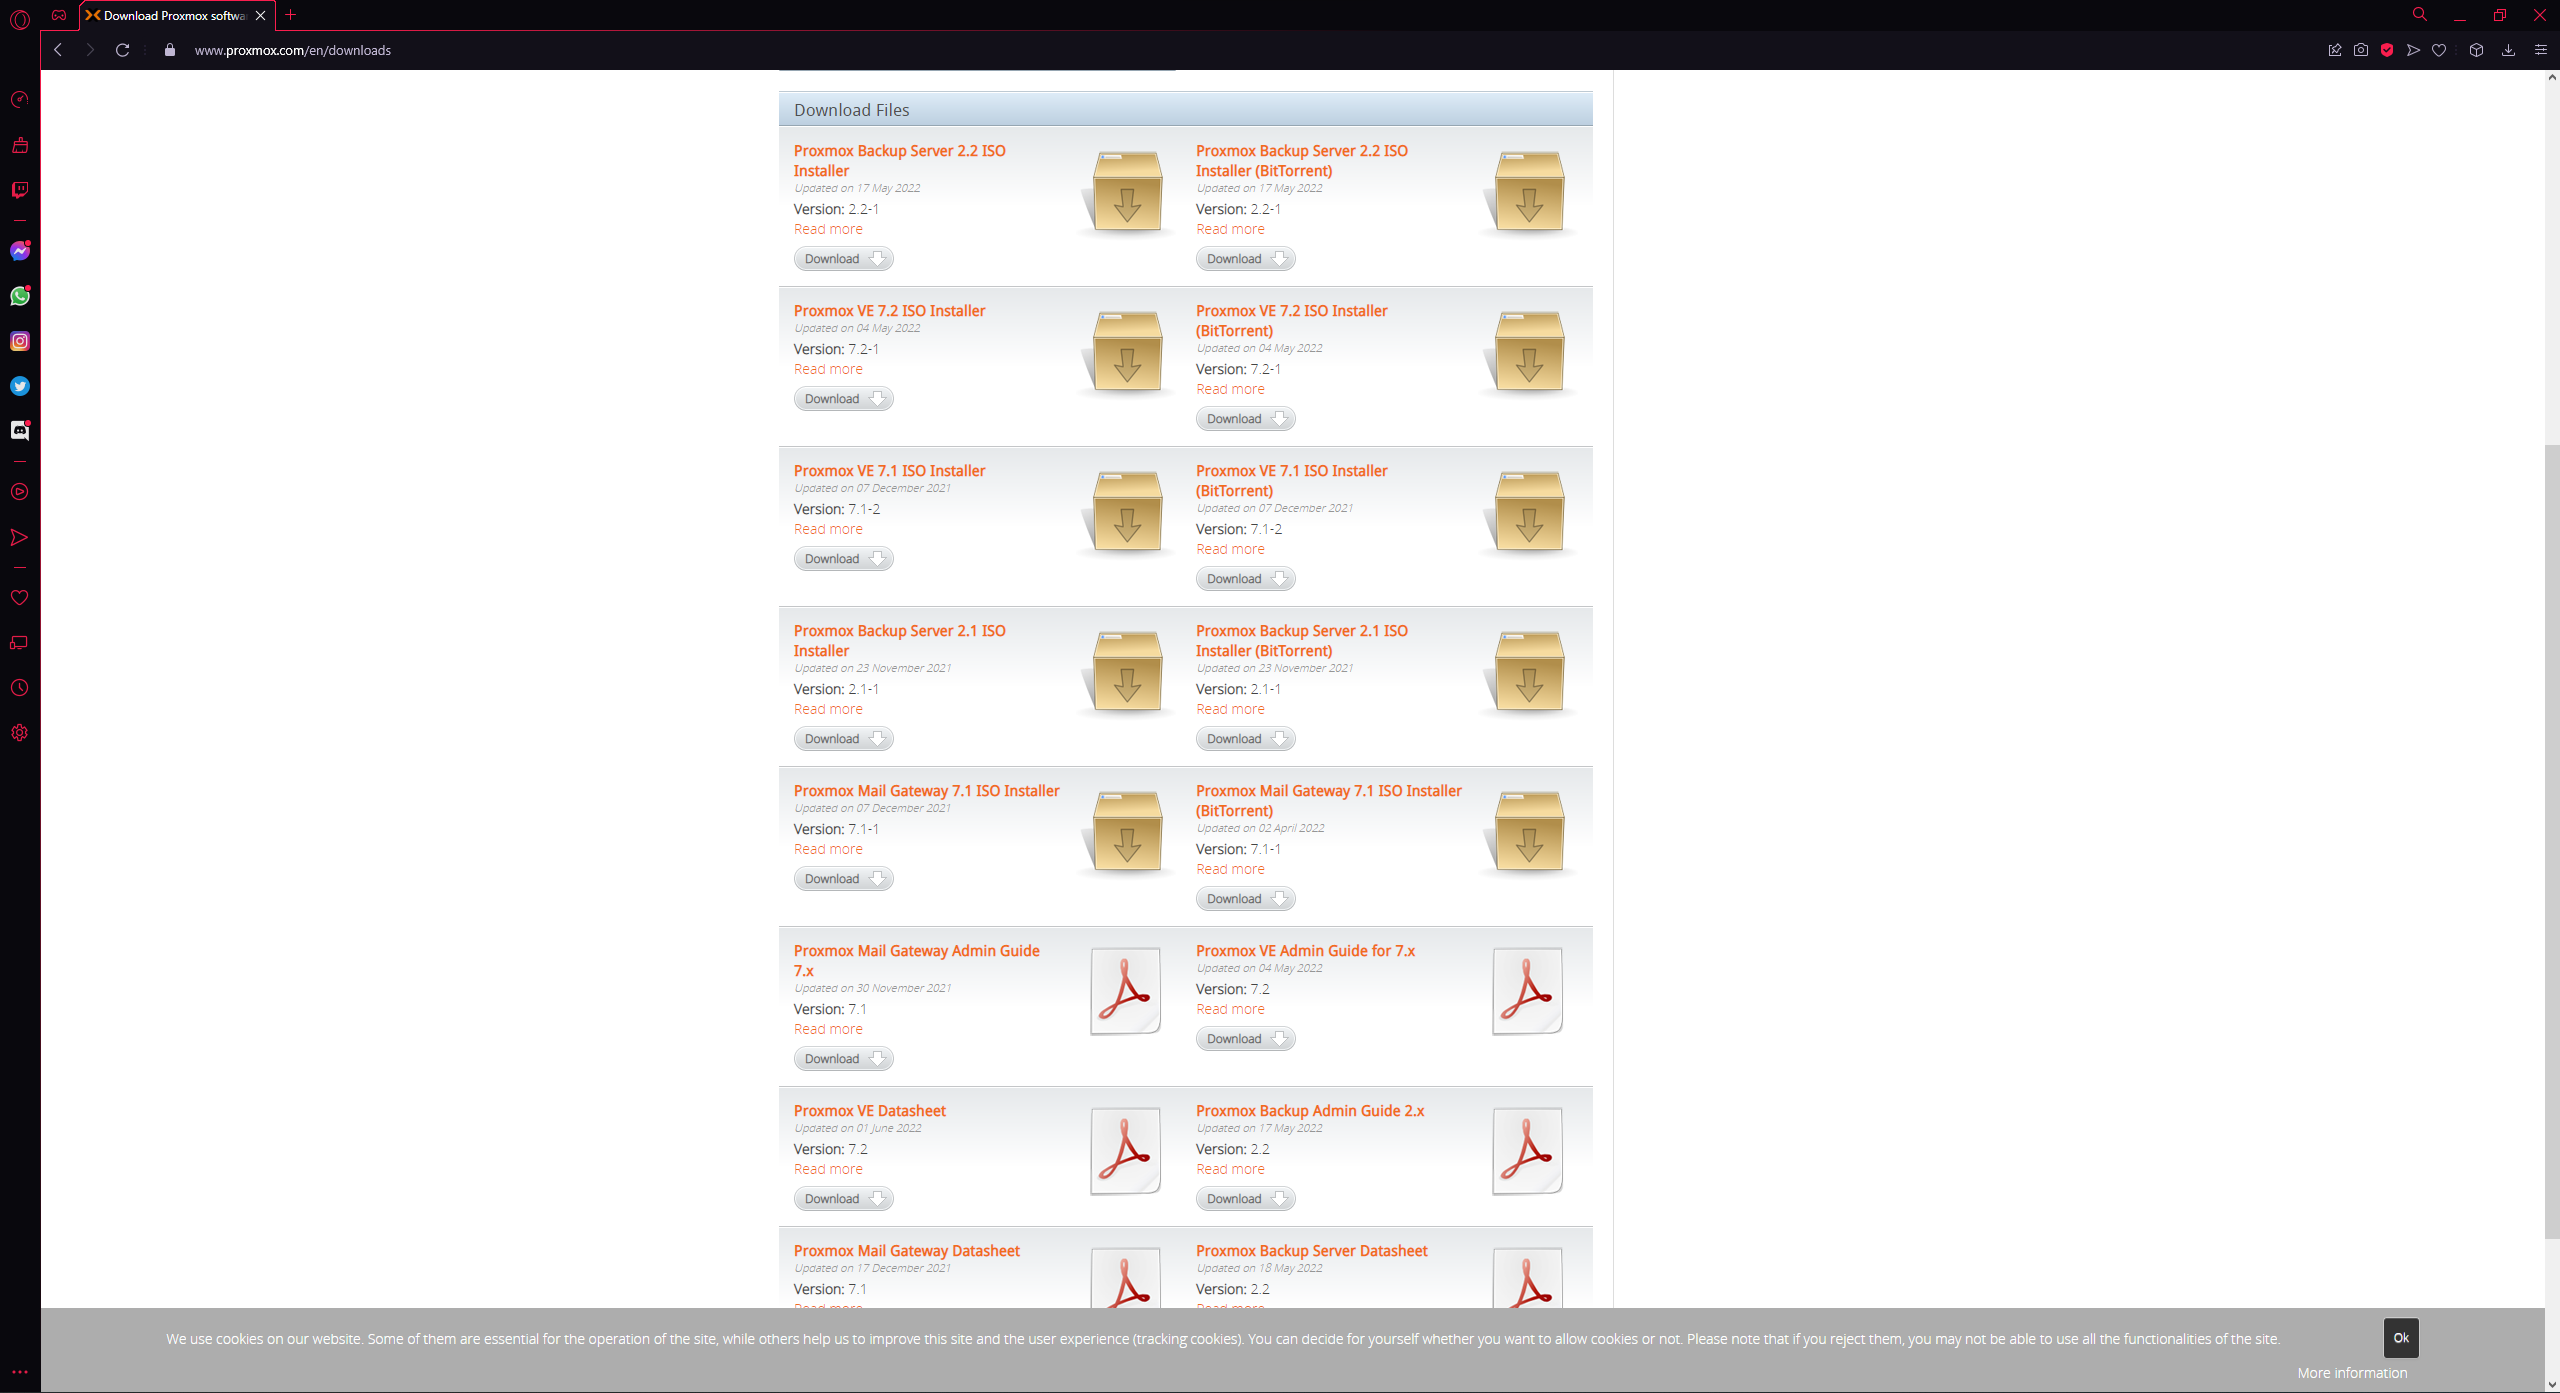
\includegraphics[width=1\linewidth]{proxmox web.png}
    \caption{web proxmox}
  \end{figure}
  \\ Setelah masuk ke website proxmox, tekan download pada salah satu list. Disarankan untuk mendownload Proxmox VE 7.1 ISO Installer
  \begin{figure}[h!]
    \centering
    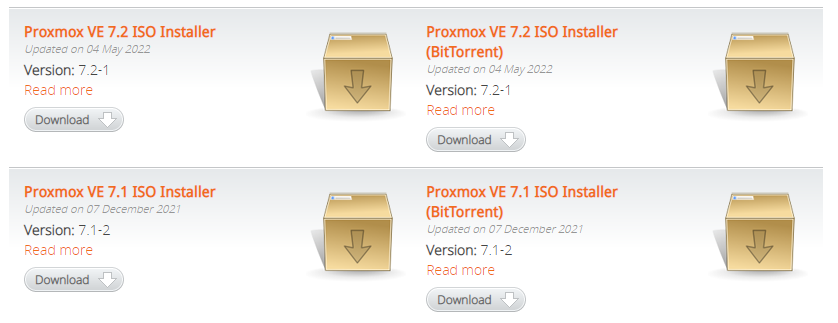
\includegraphics[width=1\linewidth]{proxmox download.png}
    \caption{download ISO}
  \end{figure}

  \newpage
  \subsection{Membuat Bootable}
  Pada proses pembuatan bootable ISO proxmox yang telah didownload akan dimasukkan ke USB flashdisk melalui proses flash menggunakan aplikasi balenaEtcher. 
  Aplikasi tersebut dapat didownload di \url{https://www.balena.io/etcher/}
  \begin{figure}[h!]
    \centering
    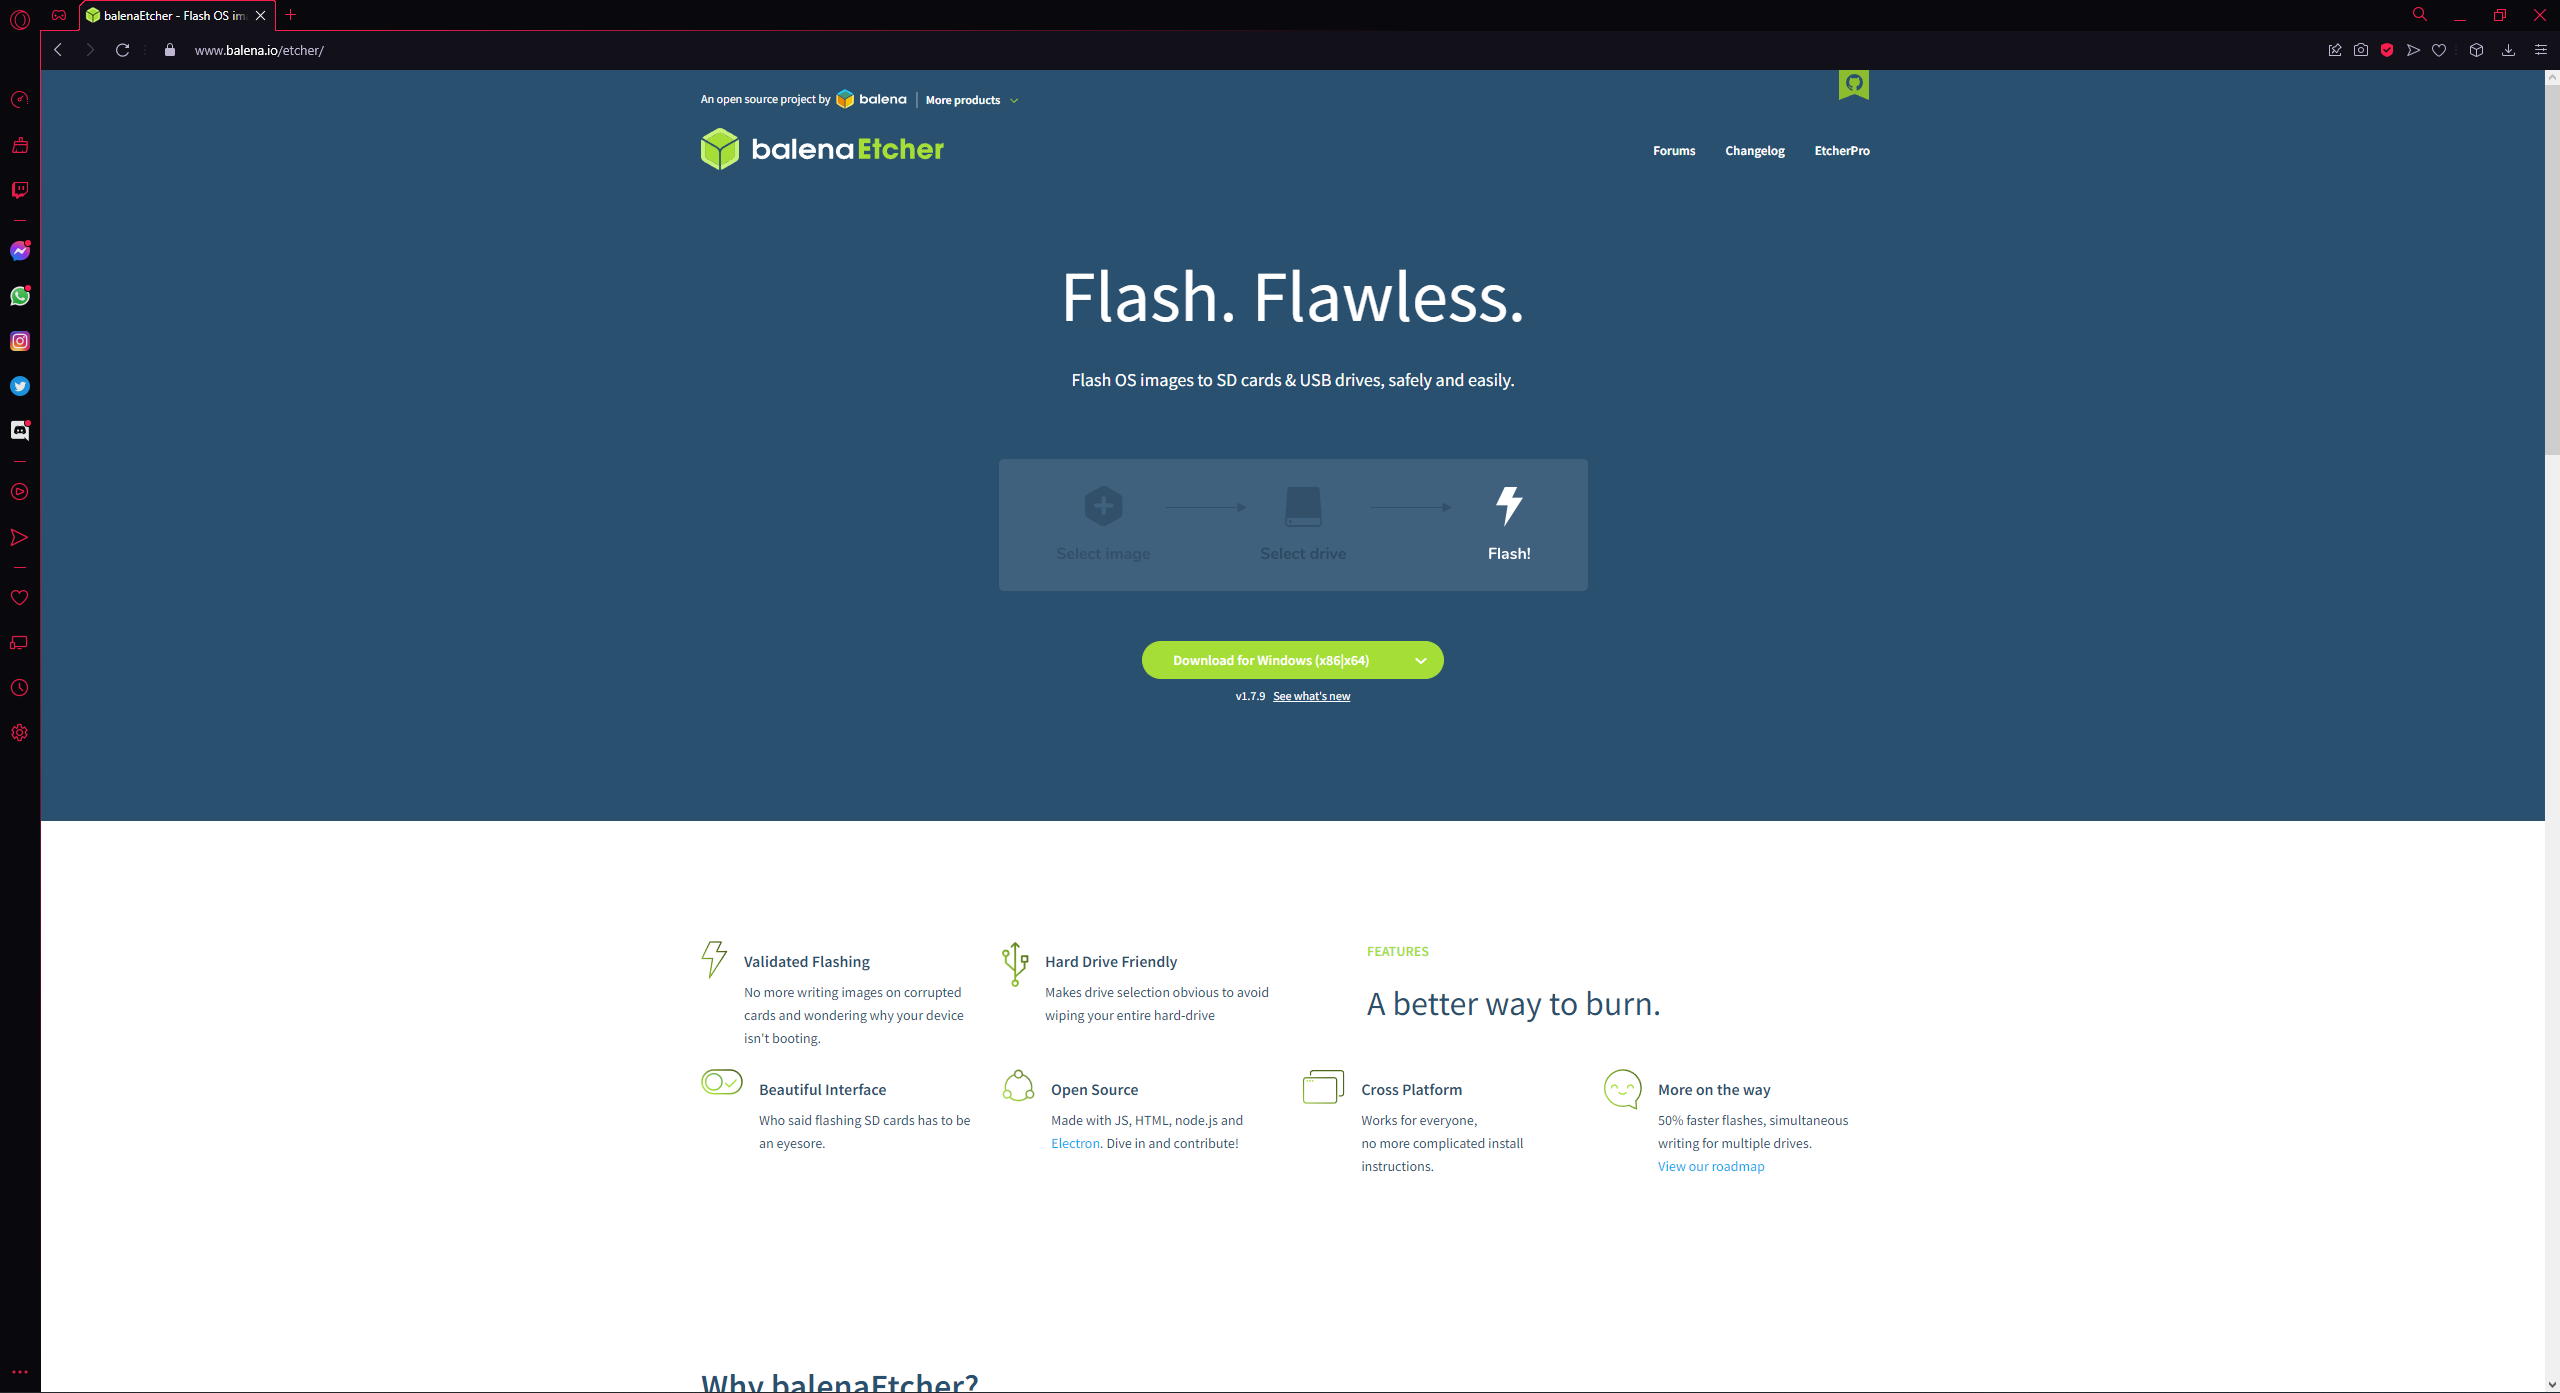
\includegraphics[width=0.9\linewidth]{balena web.png}
    \caption{web balena}
  \end{figure}
  \\ Setelah itu download aplikasi balenaEtcher sesuai sistem operasi yang digunakan. 
  Setelah proses download selesai maka lakukan instalasi aplikasi balenaEtcher,
  jika proses instalasi selesai maka akan muncul tampilan seperti berikut. Sambungkan USB flashdisk ke PC, 
  lalu pada aplikasi balenaEtcher pilih Flash from file,
  seteh itu pada Select target pilih USB flashdisk, lalu Flash!
  \begin{figure}[h!]
    \centering
    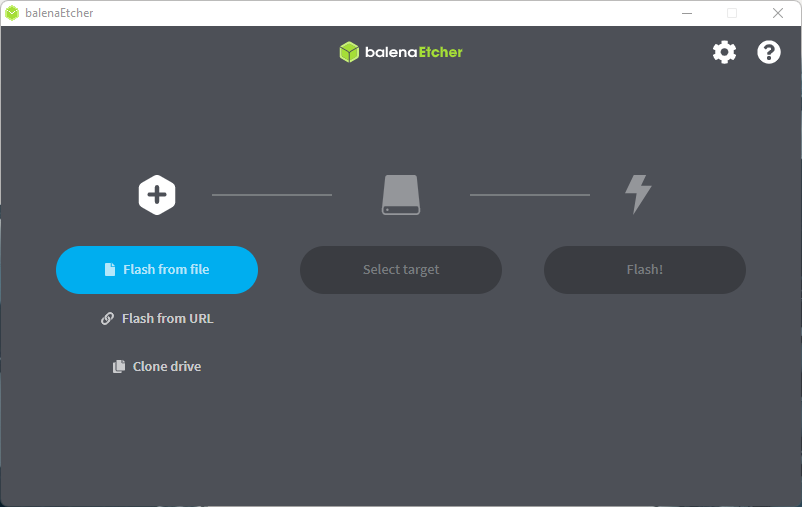
\includegraphics[width=0.75\linewidth]{balena.png}
    \caption{aplikasi balena}
  \end{figure}
  \\ Jika terdapat error pada proses bootable maka matikan terlebih dahulu windows firewall.
  \begin{figure}[h!]
    \centering
    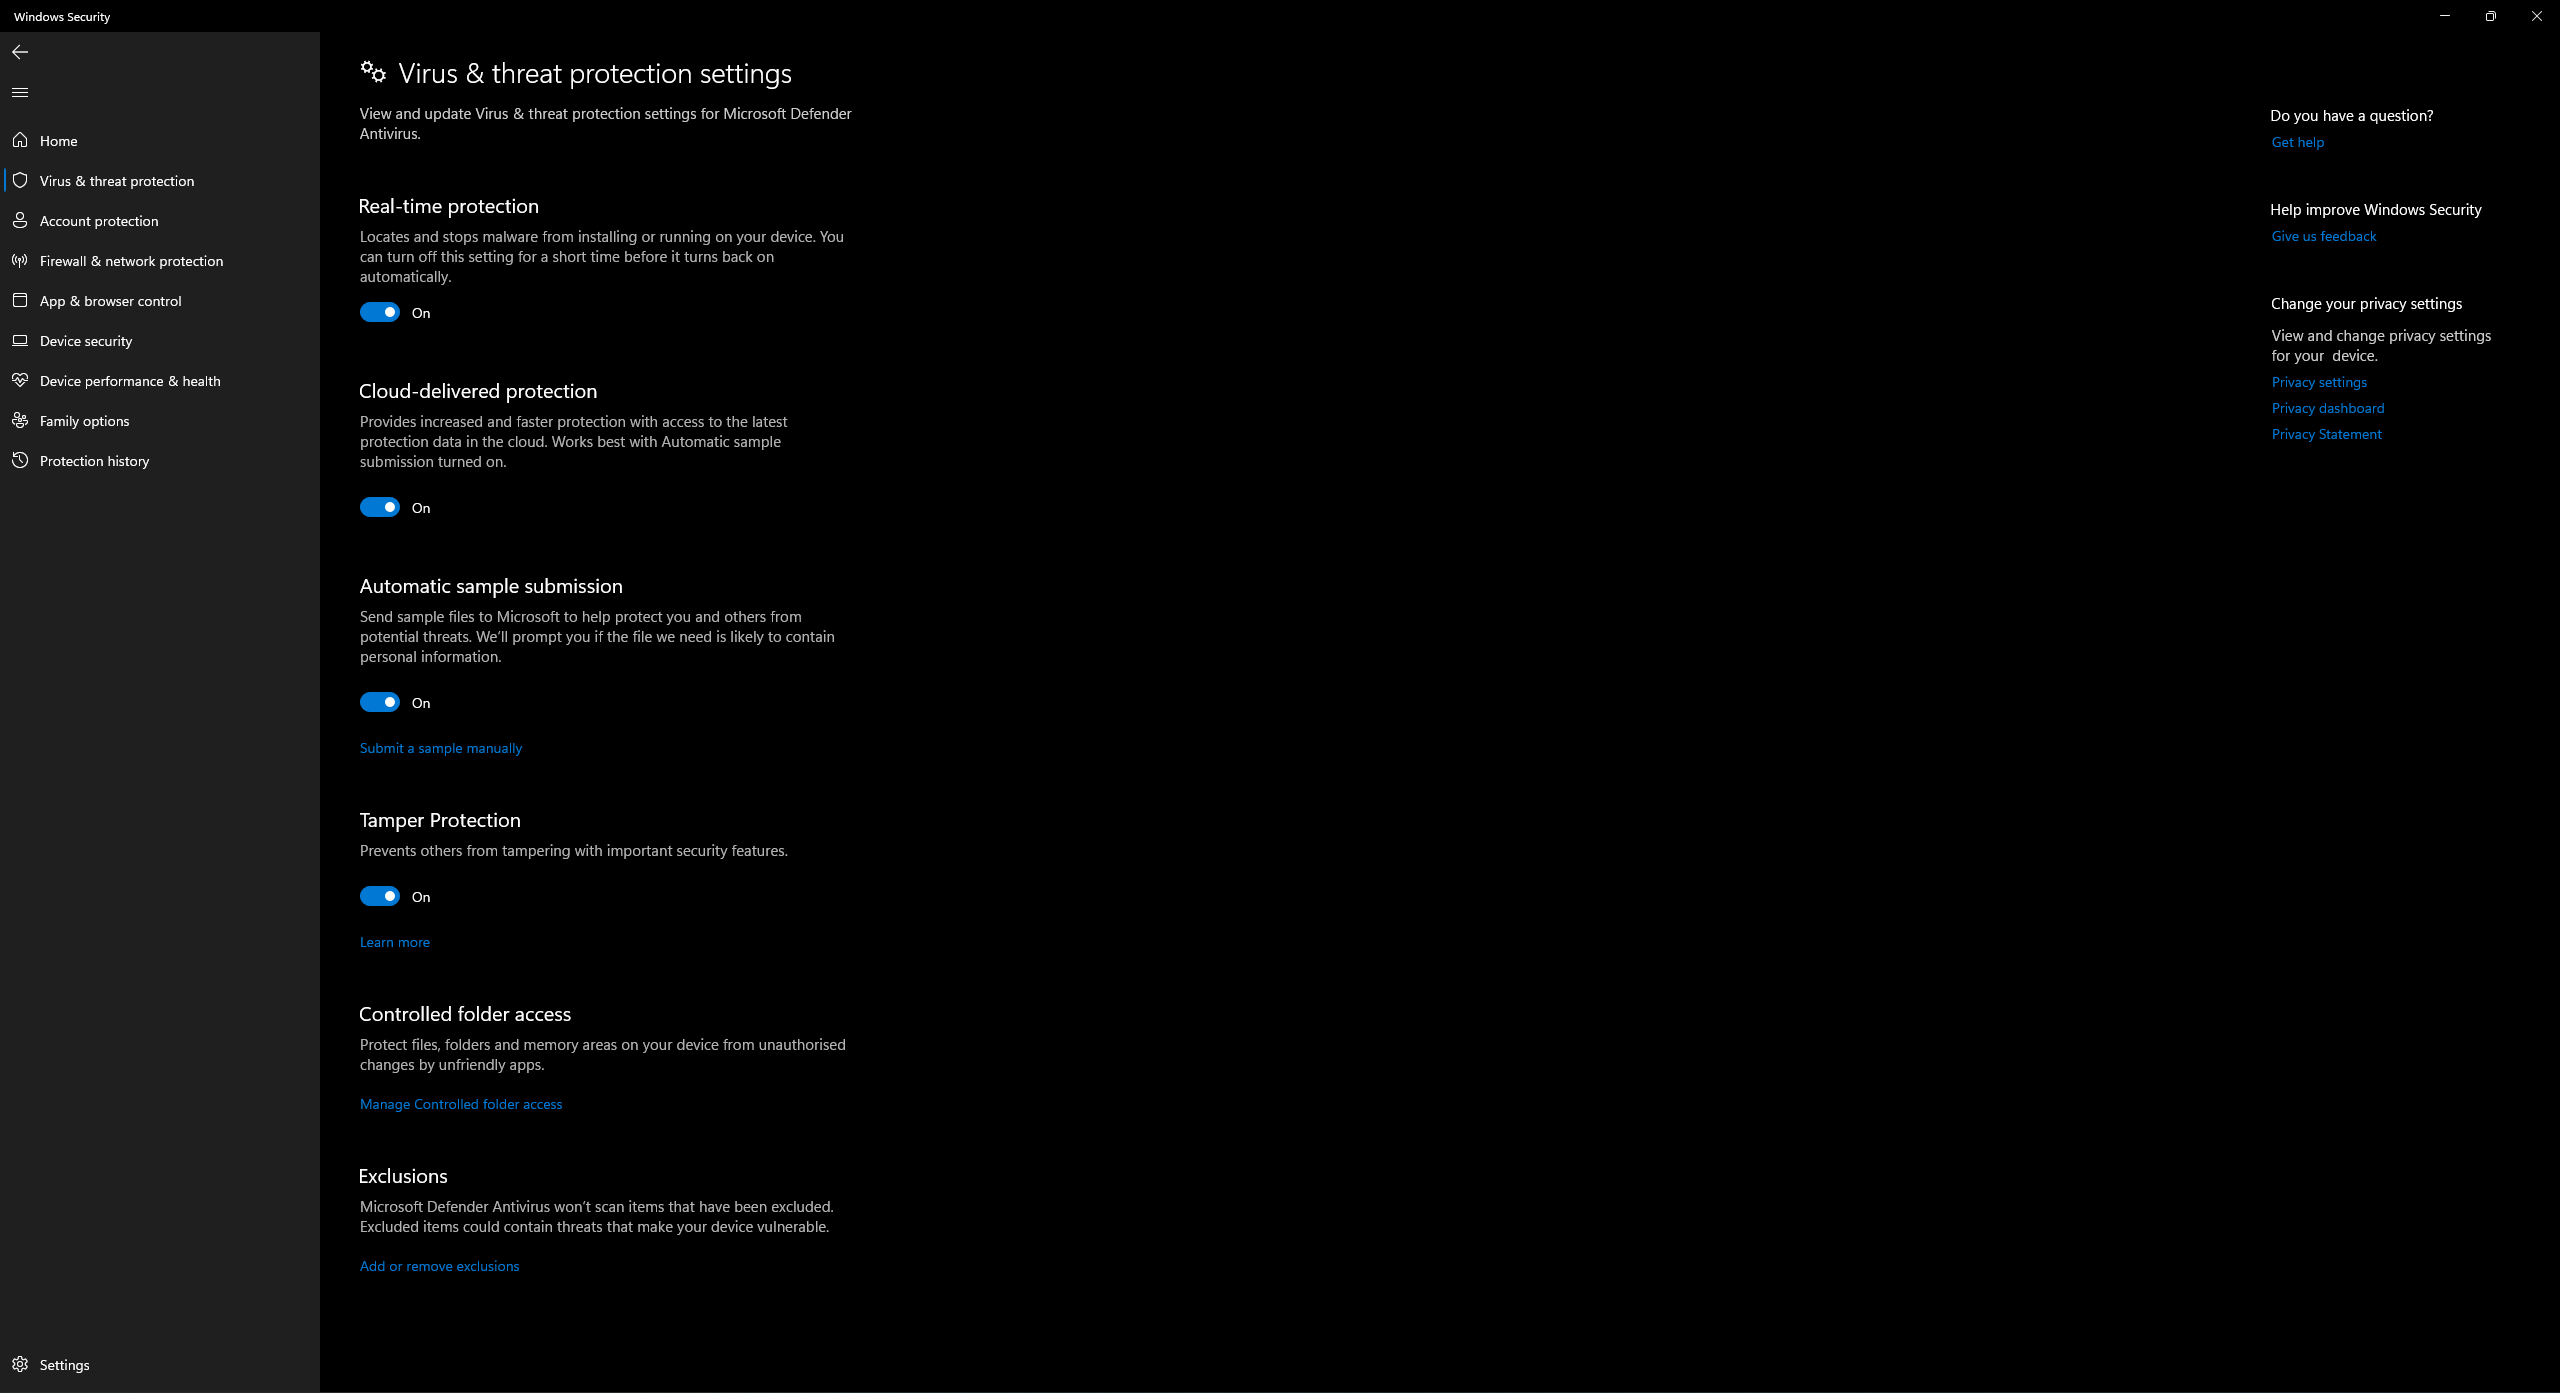
\includegraphics[width=0.7\linewidth]{firewall.png}
    \caption{firewall}
  \end{figure}
  \\ Setelah proses bootable, pasangkan USB flashdisk pada PC yang akan diinstall proxmox. Ubahlah proses Boot pada PC dengan memasuki BIOS atau UEFI,
  lalu masuk ke menu Boot atau System Configuration dan pilih Boot Order/Hard drive BBS Priorities. Pastikan Boot USB berada dipaling atas
  \newpage

  \subsection{Instalasi Proxmox}
  Setelah memasuki Boot pada USB flashdisk maka akan muncul tampilan seperti berikut. Berikut merupakan langkah - langkah instalasi :
  \begin{enumerate}
    \item Pilih Install Proxmox VE
    \begin{figure}[h!]
      \centering
      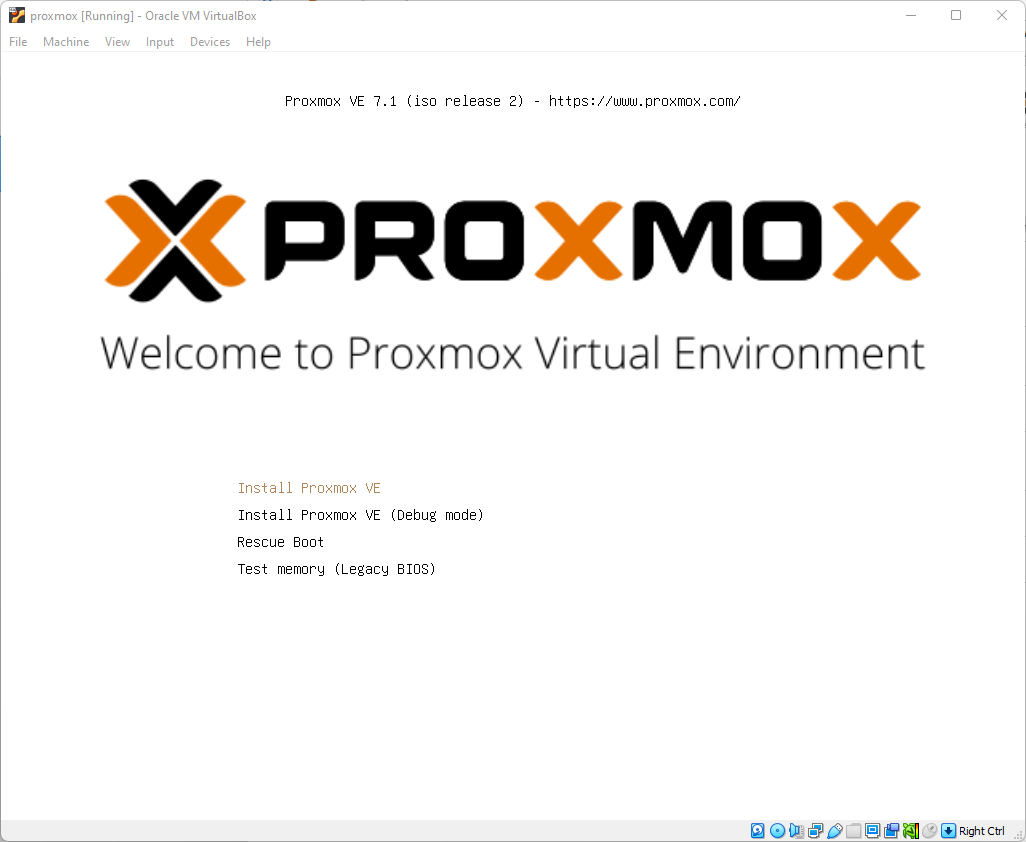
\includegraphics[width=0.7\linewidth]{proxmox 1.png}
      \caption{Proxmox 1}
    \end{figure}
    \newpage
    \item Tekan OK
    \begin{figure}[h!]
      \centering
      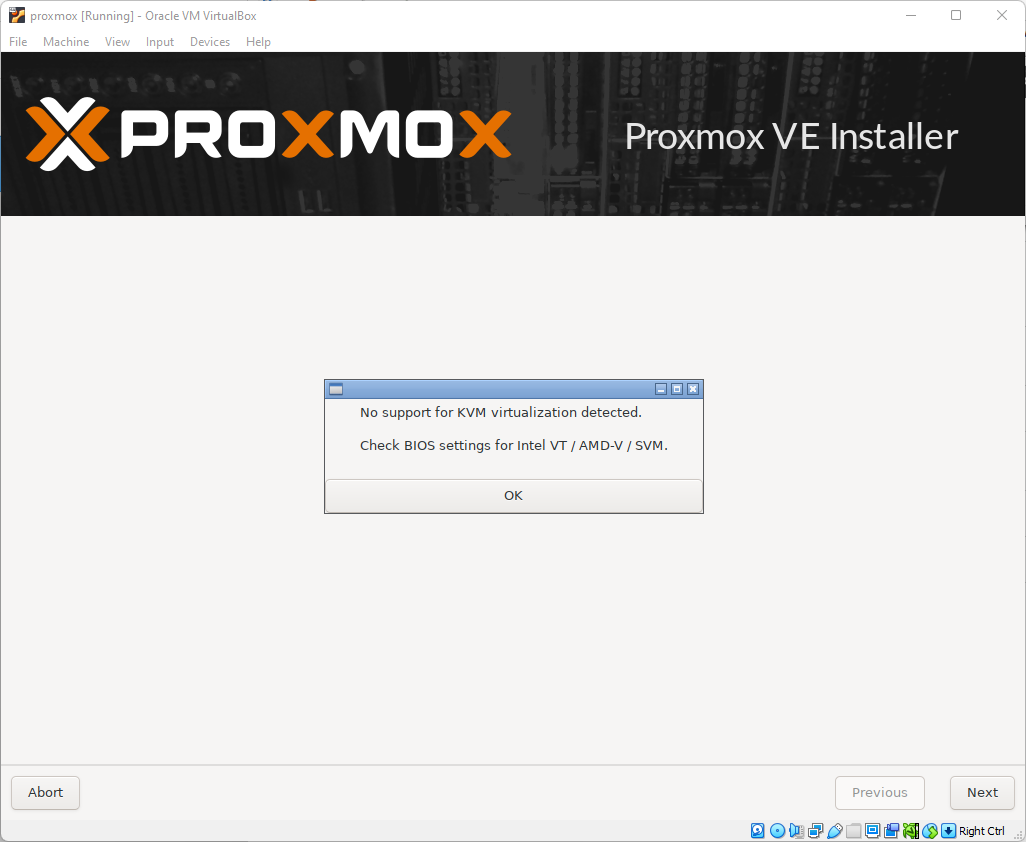
\includegraphics[width=0.7\linewidth]{proxmox 2.png}
      \caption{Proxmox 2}
    \end{figure}
    \item Tekan I agree
    \begin{figure}[h!]
      \centering
      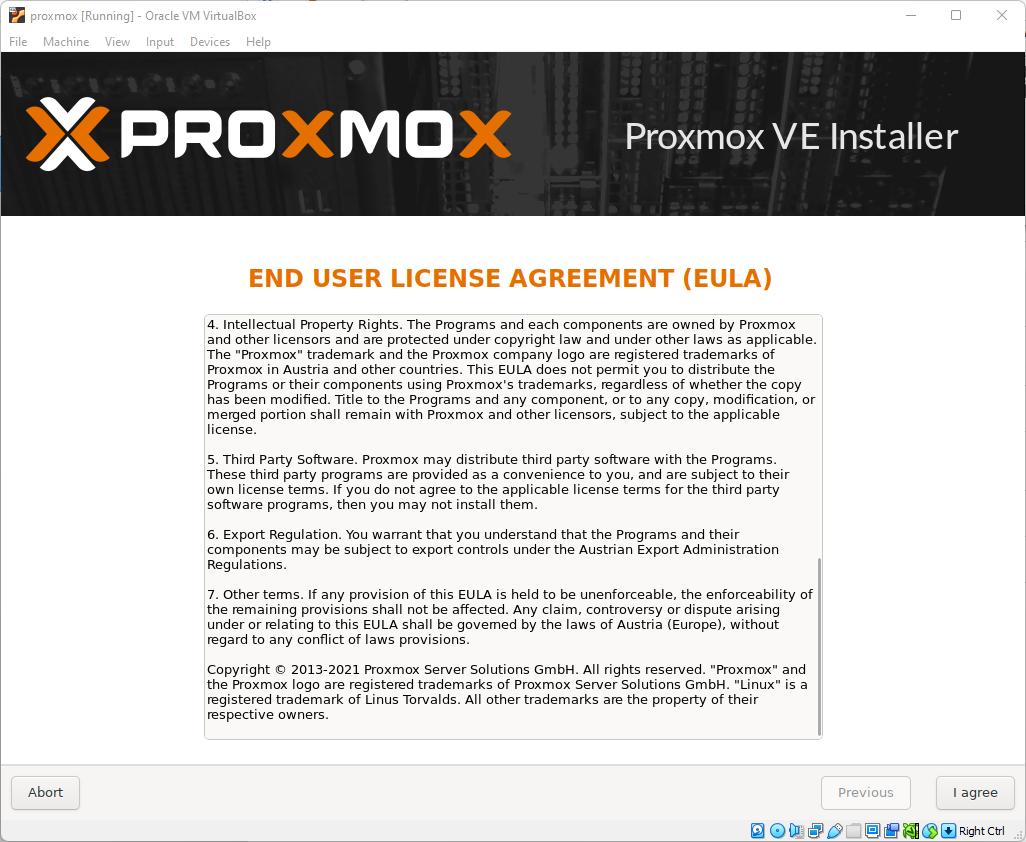
\includegraphics[width=0.7\linewidth]{proxmox 3.png}
      \caption{Proxmox 3}
    \end{figure}
    \newpage
    \item Pilih Target harddisk lalu tekan Next
    \begin{figure}[h!]
      \centering
      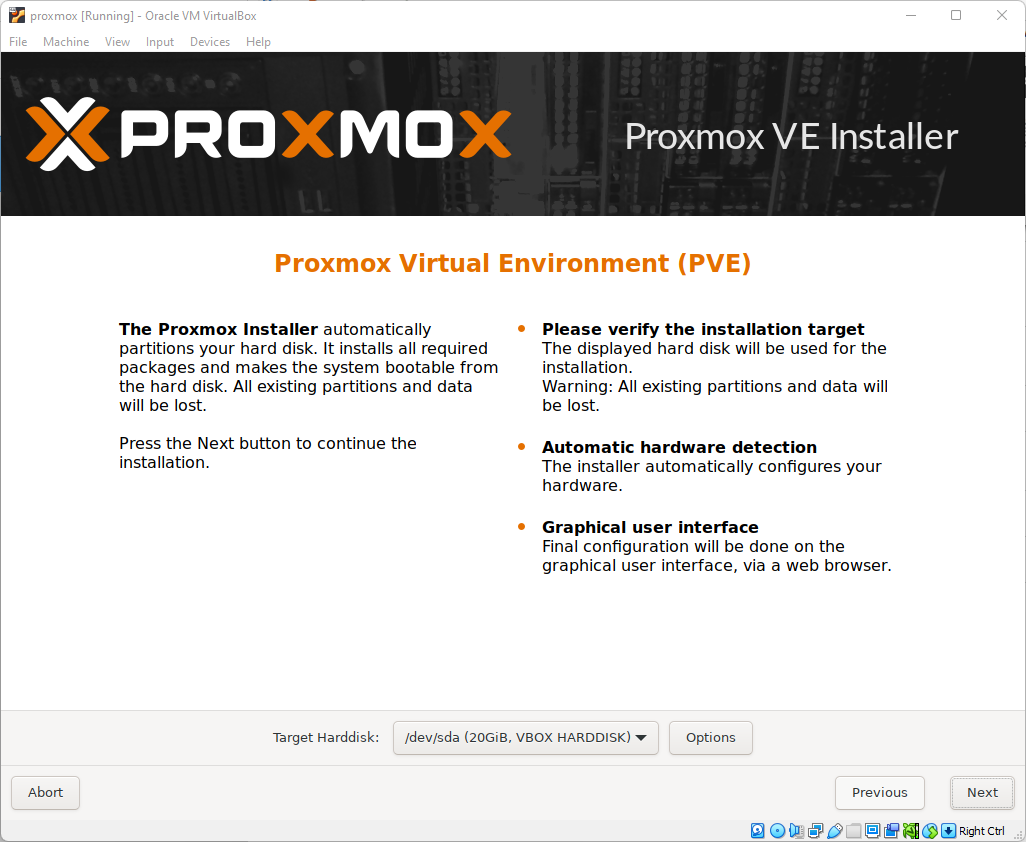
\includegraphics[width=0.7\linewidth]{proxmox 4.png}
      \caption{Proxmox 4}
    \end{figure}
    \item Pilih negara, zona waktu dan keyboard layout. Untuk keyboard layout biarkan saja menjadi U. S. English
    \begin{figure}[h!]
      \centering
      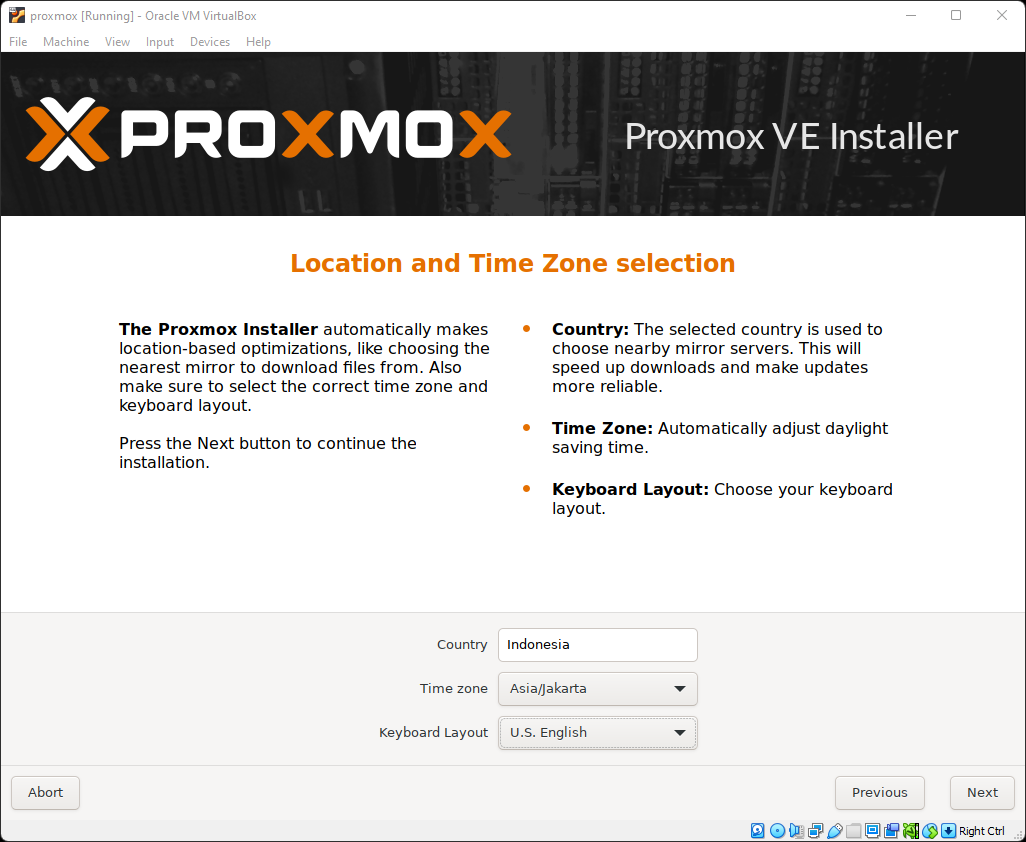
\includegraphics[width=0.7\linewidth]{proxmox 5.png}
      \caption{Proxmox 5}
    \end{figure}
    \newpage
    \item Masukkan password dan email
    \begin{figure}[h!]
      \centering
      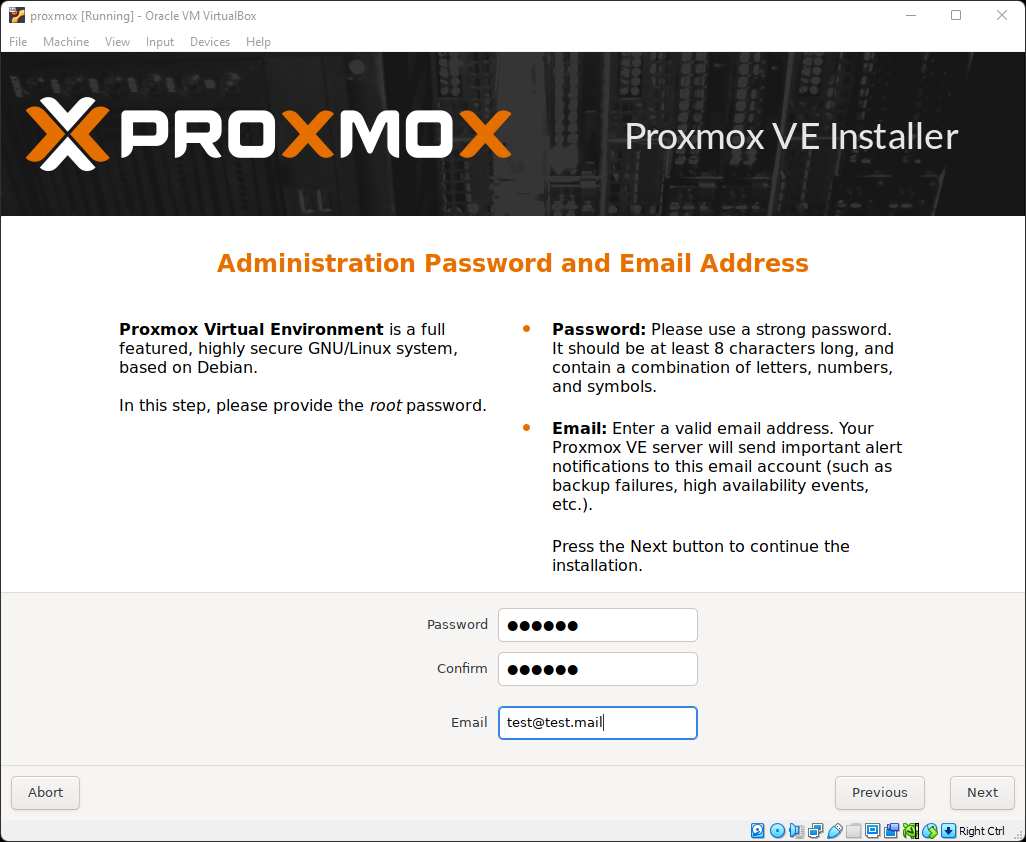
\includegraphics[width=0.7\linewidth]{proxmox 6.png}
      \caption{Proxmox 6}
    \end{figure}
    \item Masukkan hostname, IP Address, Gateway dan DNS Server
    \begin{figure}[h!]
      \centering
      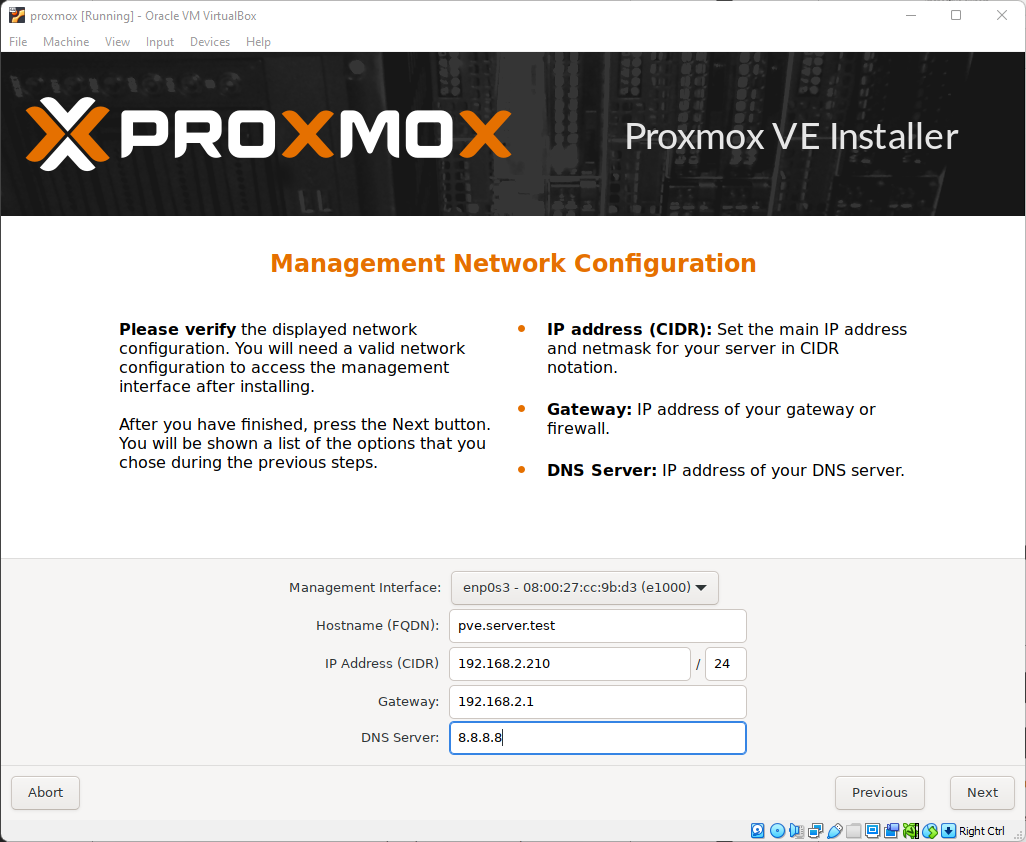
\includegraphics[width=0.7\linewidth]{proxmox 7.png}
      \caption{Proxmox 7}
    \end{figure}
    \newpage
    \item Berikut ini merupakan tampilan konfirmasi, jika ada yang tidak sesuai maka tekan tombol Previous, dan jika sudah benar maka tekan tombol Install
    \begin{figure}[h!]
      \centering
      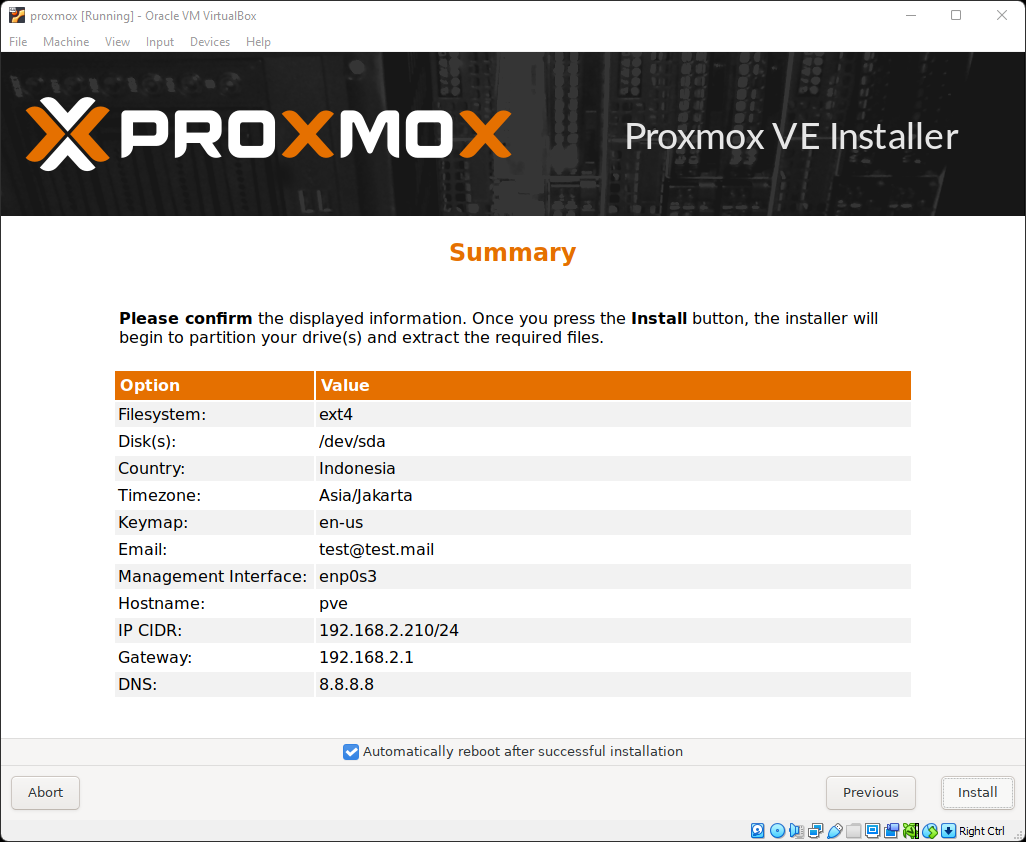
\includegraphics[width=0.7\linewidth]{proxmox 8.png}
      \caption{Proxmox 8}
    \end{figure}
    \item Berikut tampilan server jika telah berhasil di install
    \begin{figure}[h!]
      \centering
      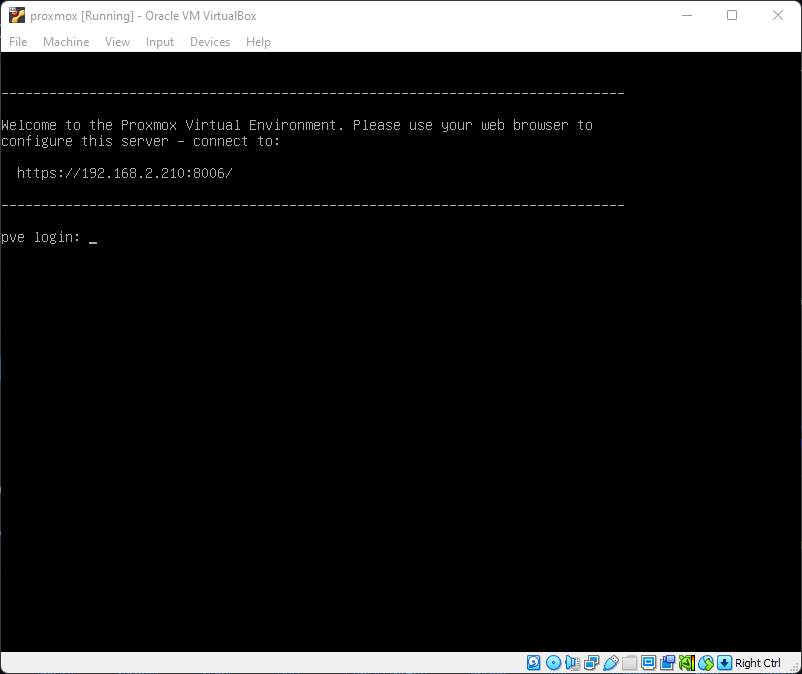
\includegraphics[width=0.7\linewidth]{proxmox 9.png}
      \caption{Proxmox 9}
    \end{figure}
  \end{enumerate}
  \newpage

  \section{Proxmox}
  \subsection{Proxmox Web GUI}
  Setelah melakukan proses instalasi, pastikan server terhubung dengan jaringan lokal,
  dengan cara menggunakan perintah ping pada PC.
  \begin{figure}[h!]
    \centering
    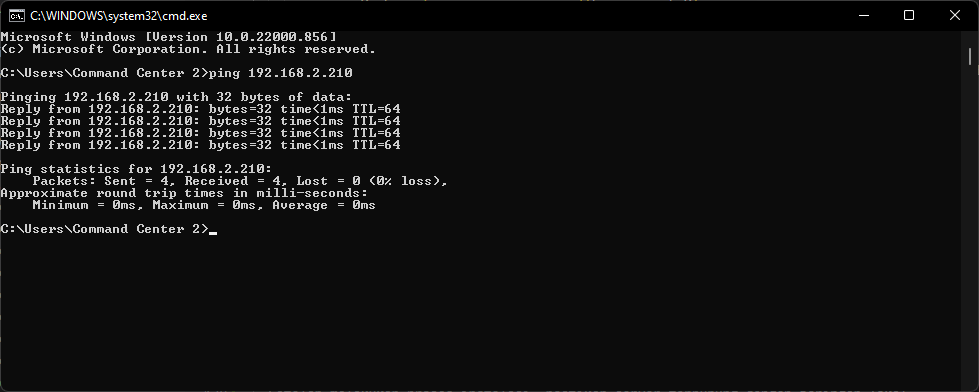
\includegraphics[width=0.7\linewidth]{cmd.png}
    \caption{Ping}
  \end{figure}
  \\ Setelah dipastikan terhubung, buka browser lalu ketikkan url proxmox seperti berikut pada search bar.
  Url ditulis menggunakan https terlebih dahulu lalu dilanjut dengan ip address server dan port 8006. Sebagai contoh
  \url{https://192.168.2.210:8006}
  \begin{figure}[h!]
    \centering
    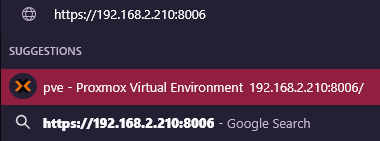
\includegraphics[width=0.7\linewidth]{url proxmox.png}
    \caption{Url Proxmox}
  \end{figure}
  \newpage
  Berikut merupakan tampilan login proxmox. Masukkan user dan password yang telah diatur.
  \begin{figure}[h!]
    \centering
    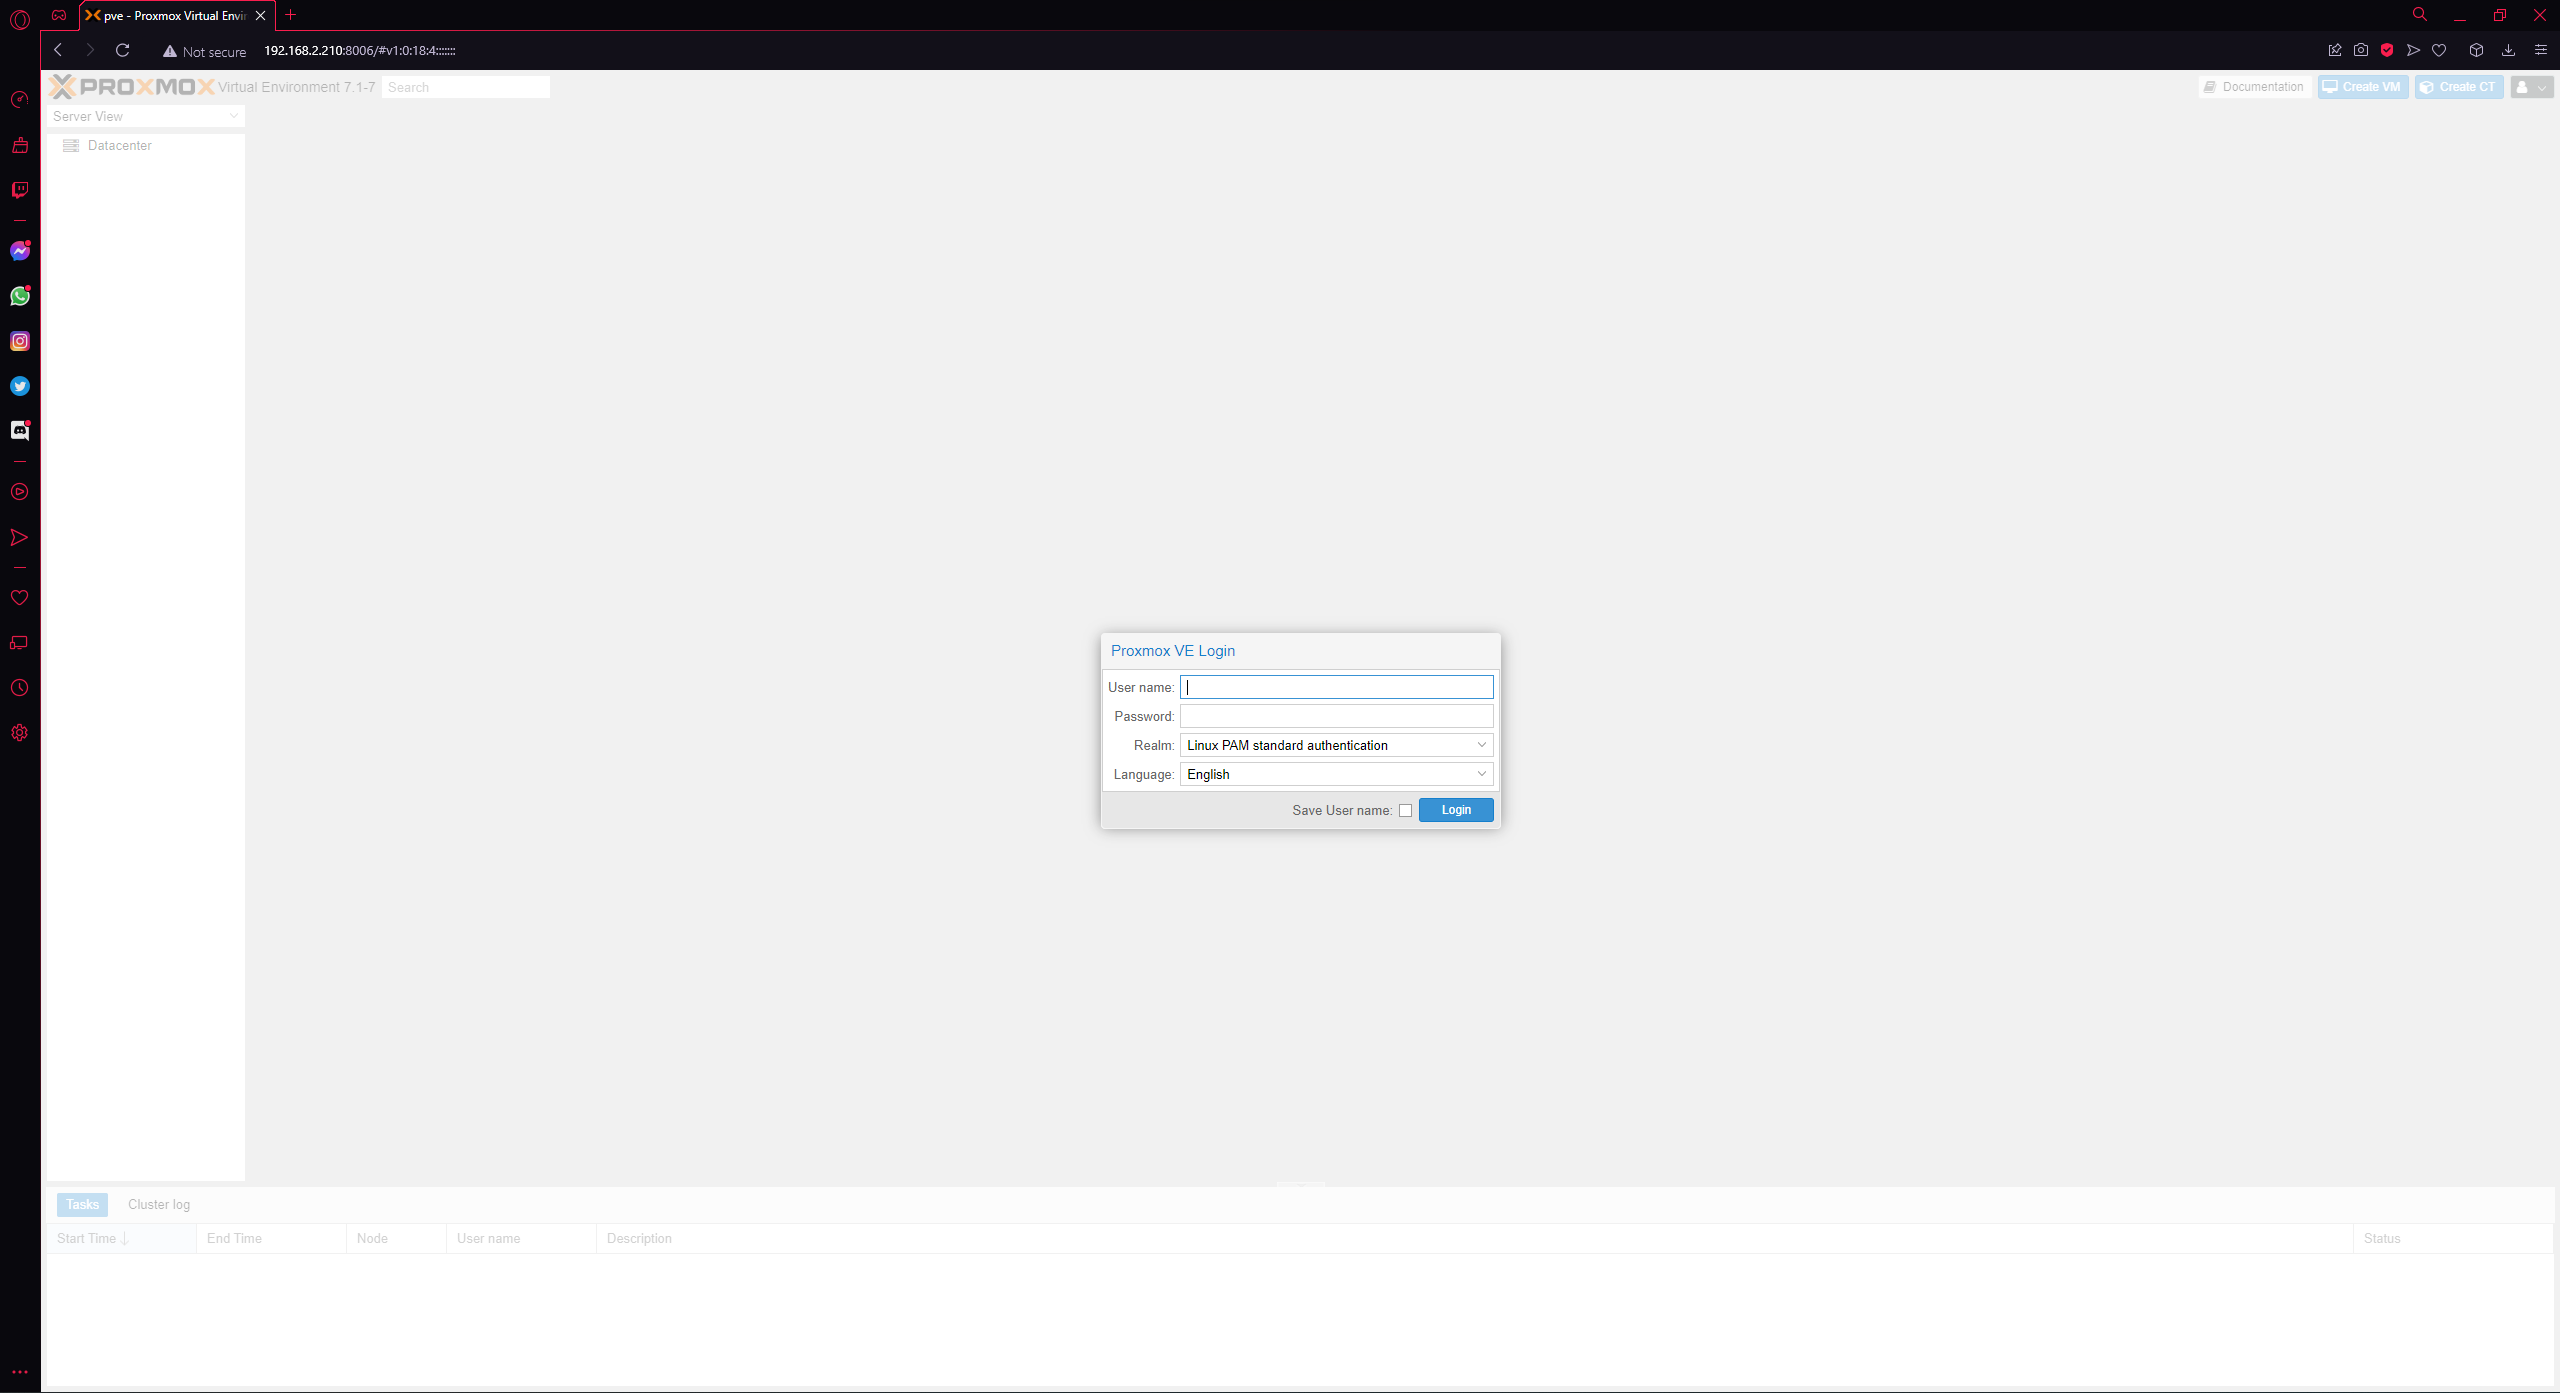
\includegraphics[width=0.7\linewidth]{login proxmox 1.png}
    \caption{Login Proxmox 1}
  \end{figure}
  \\ Tekan tombol OK jika muncul tampilan seperti berikut.
  \begin{figure}[h!]
    \centering
    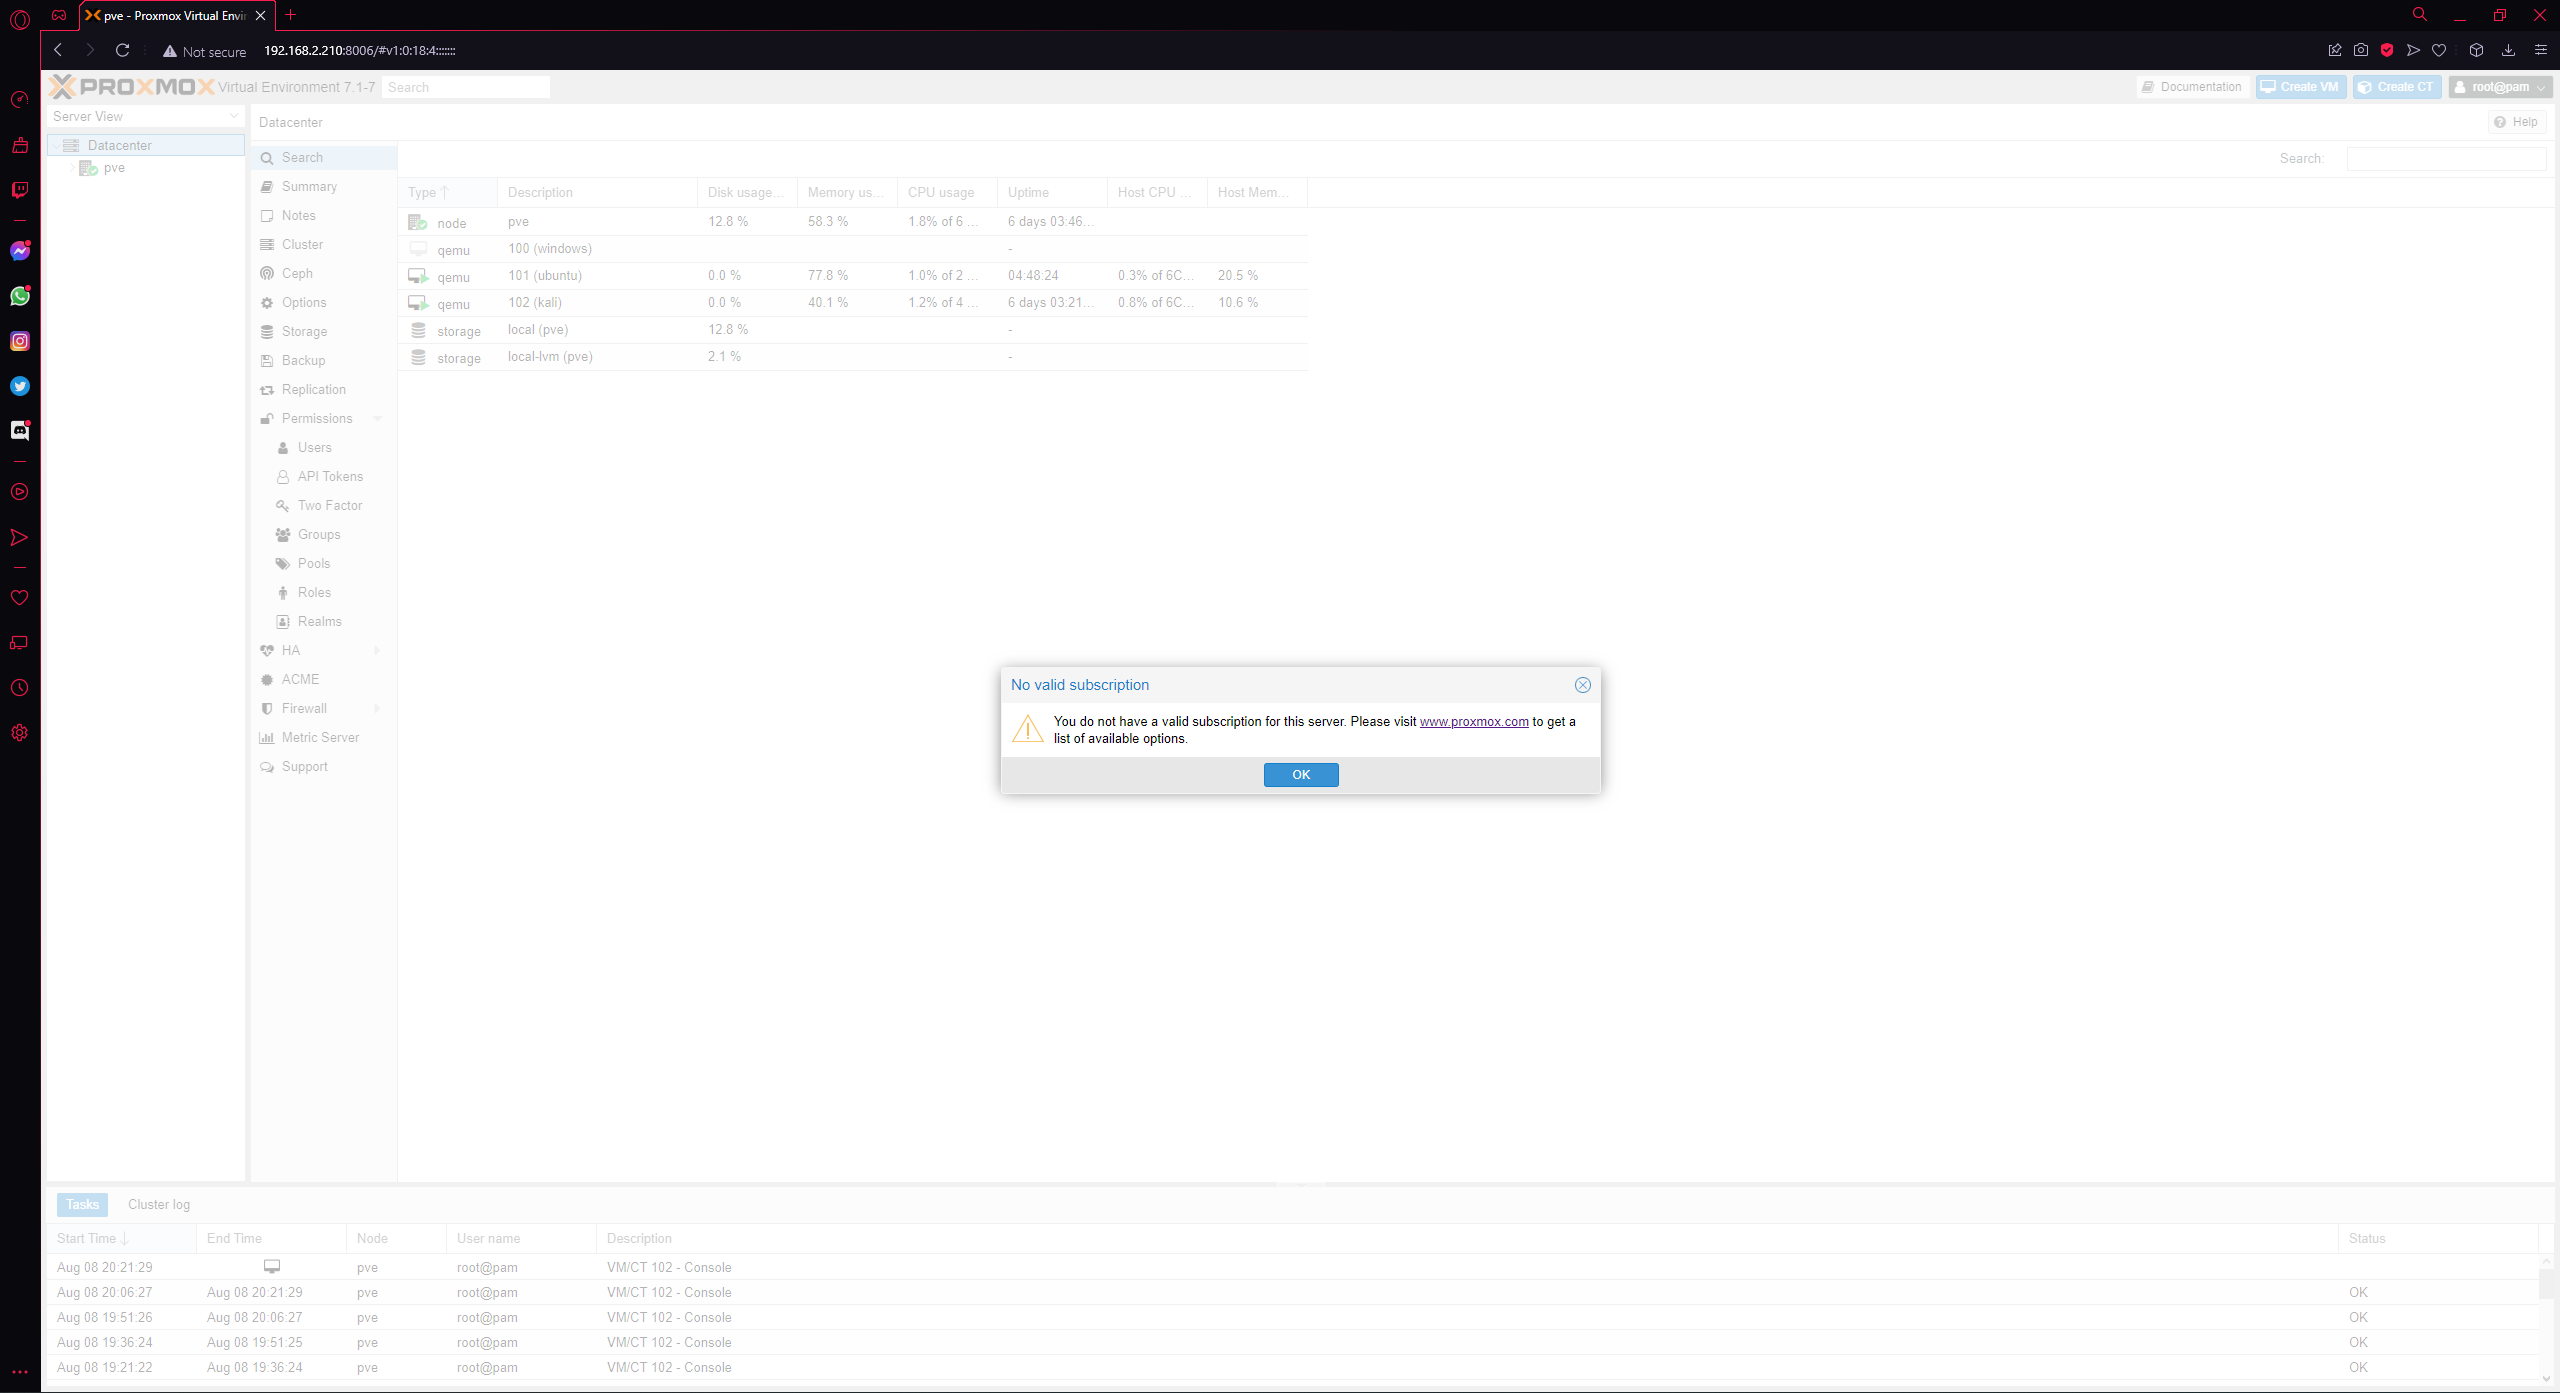
\includegraphics[width=0.7\linewidth]{login proxmox 2.png}
    \caption{Login Proxmox 2}
  \end{figure}
  \newpage
  
  \subsection{Upload ISO Image}
  Setelah masuk ke web GUI proxmox, pada panel sebelah kiri terdapat list Datacenter klik list tersebut,
  maka akan muncul tampilan seperti berikut.
  \begin{figure}[h!]
    \centering
    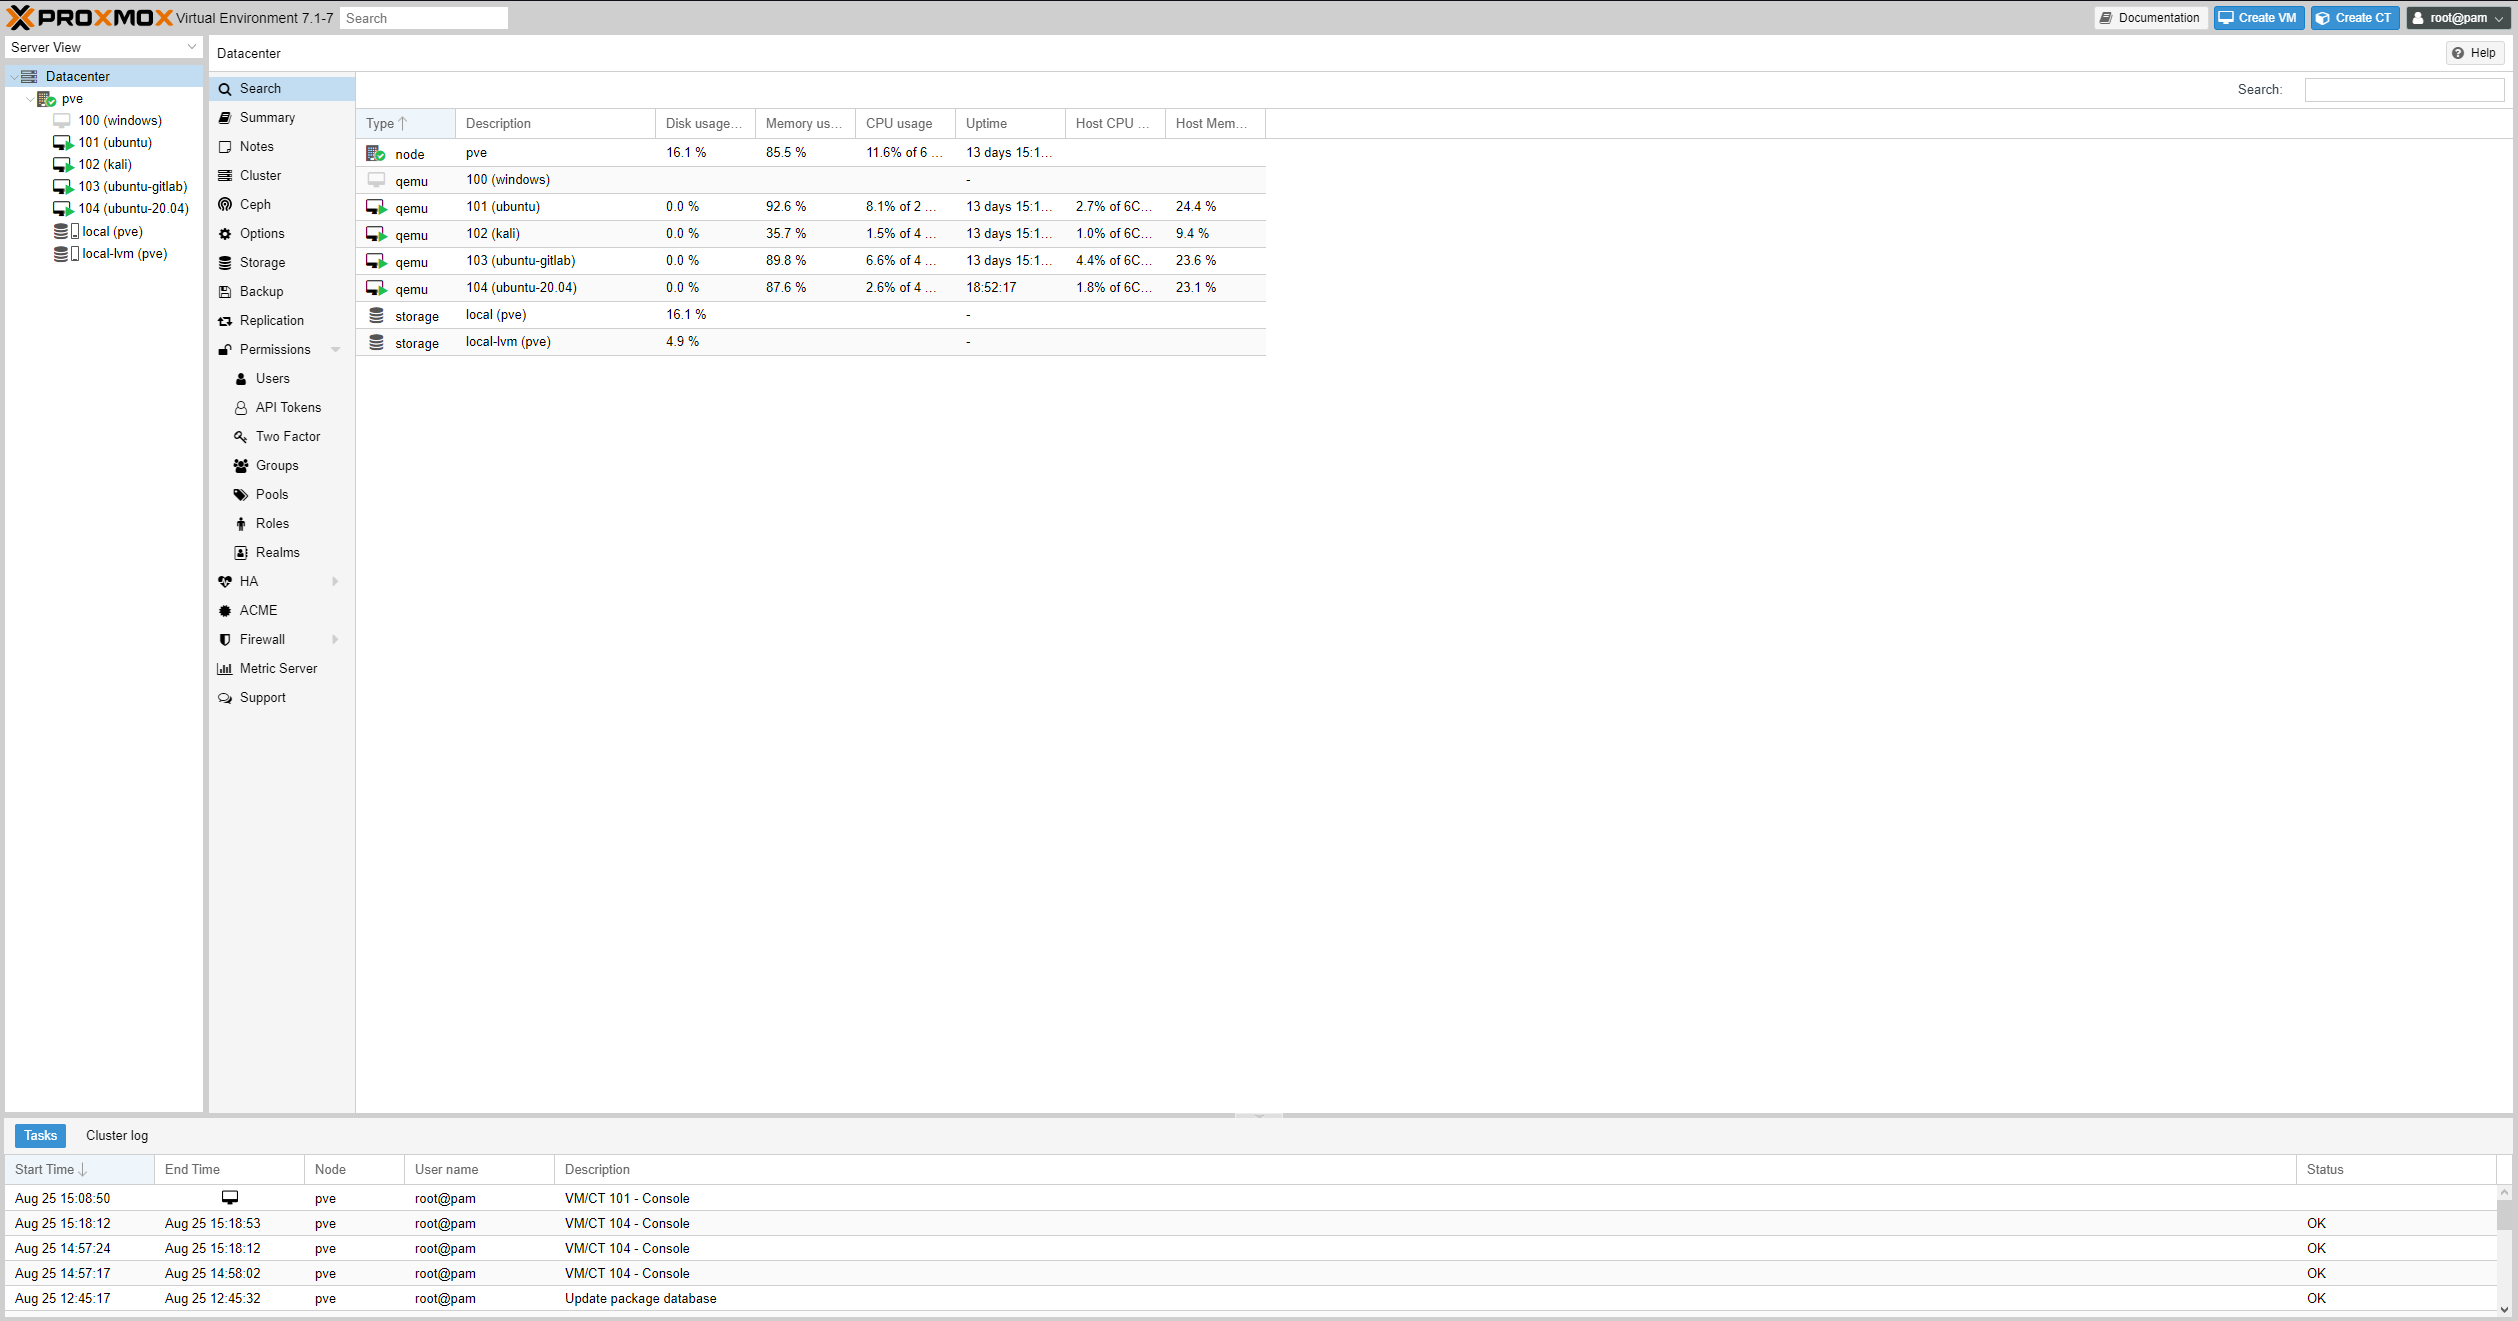
\includegraphics[width=0.7\linewidth]{datacenter.png}
    \caption{Datacenter}
  \end{figure}
  \\ Klik 2 kali pada storage local (pve), setelah itu pilih menu ISO Images, maka akan muncul tampilan seperti berikut.
  \begin{figure}[h!]
    \centering
    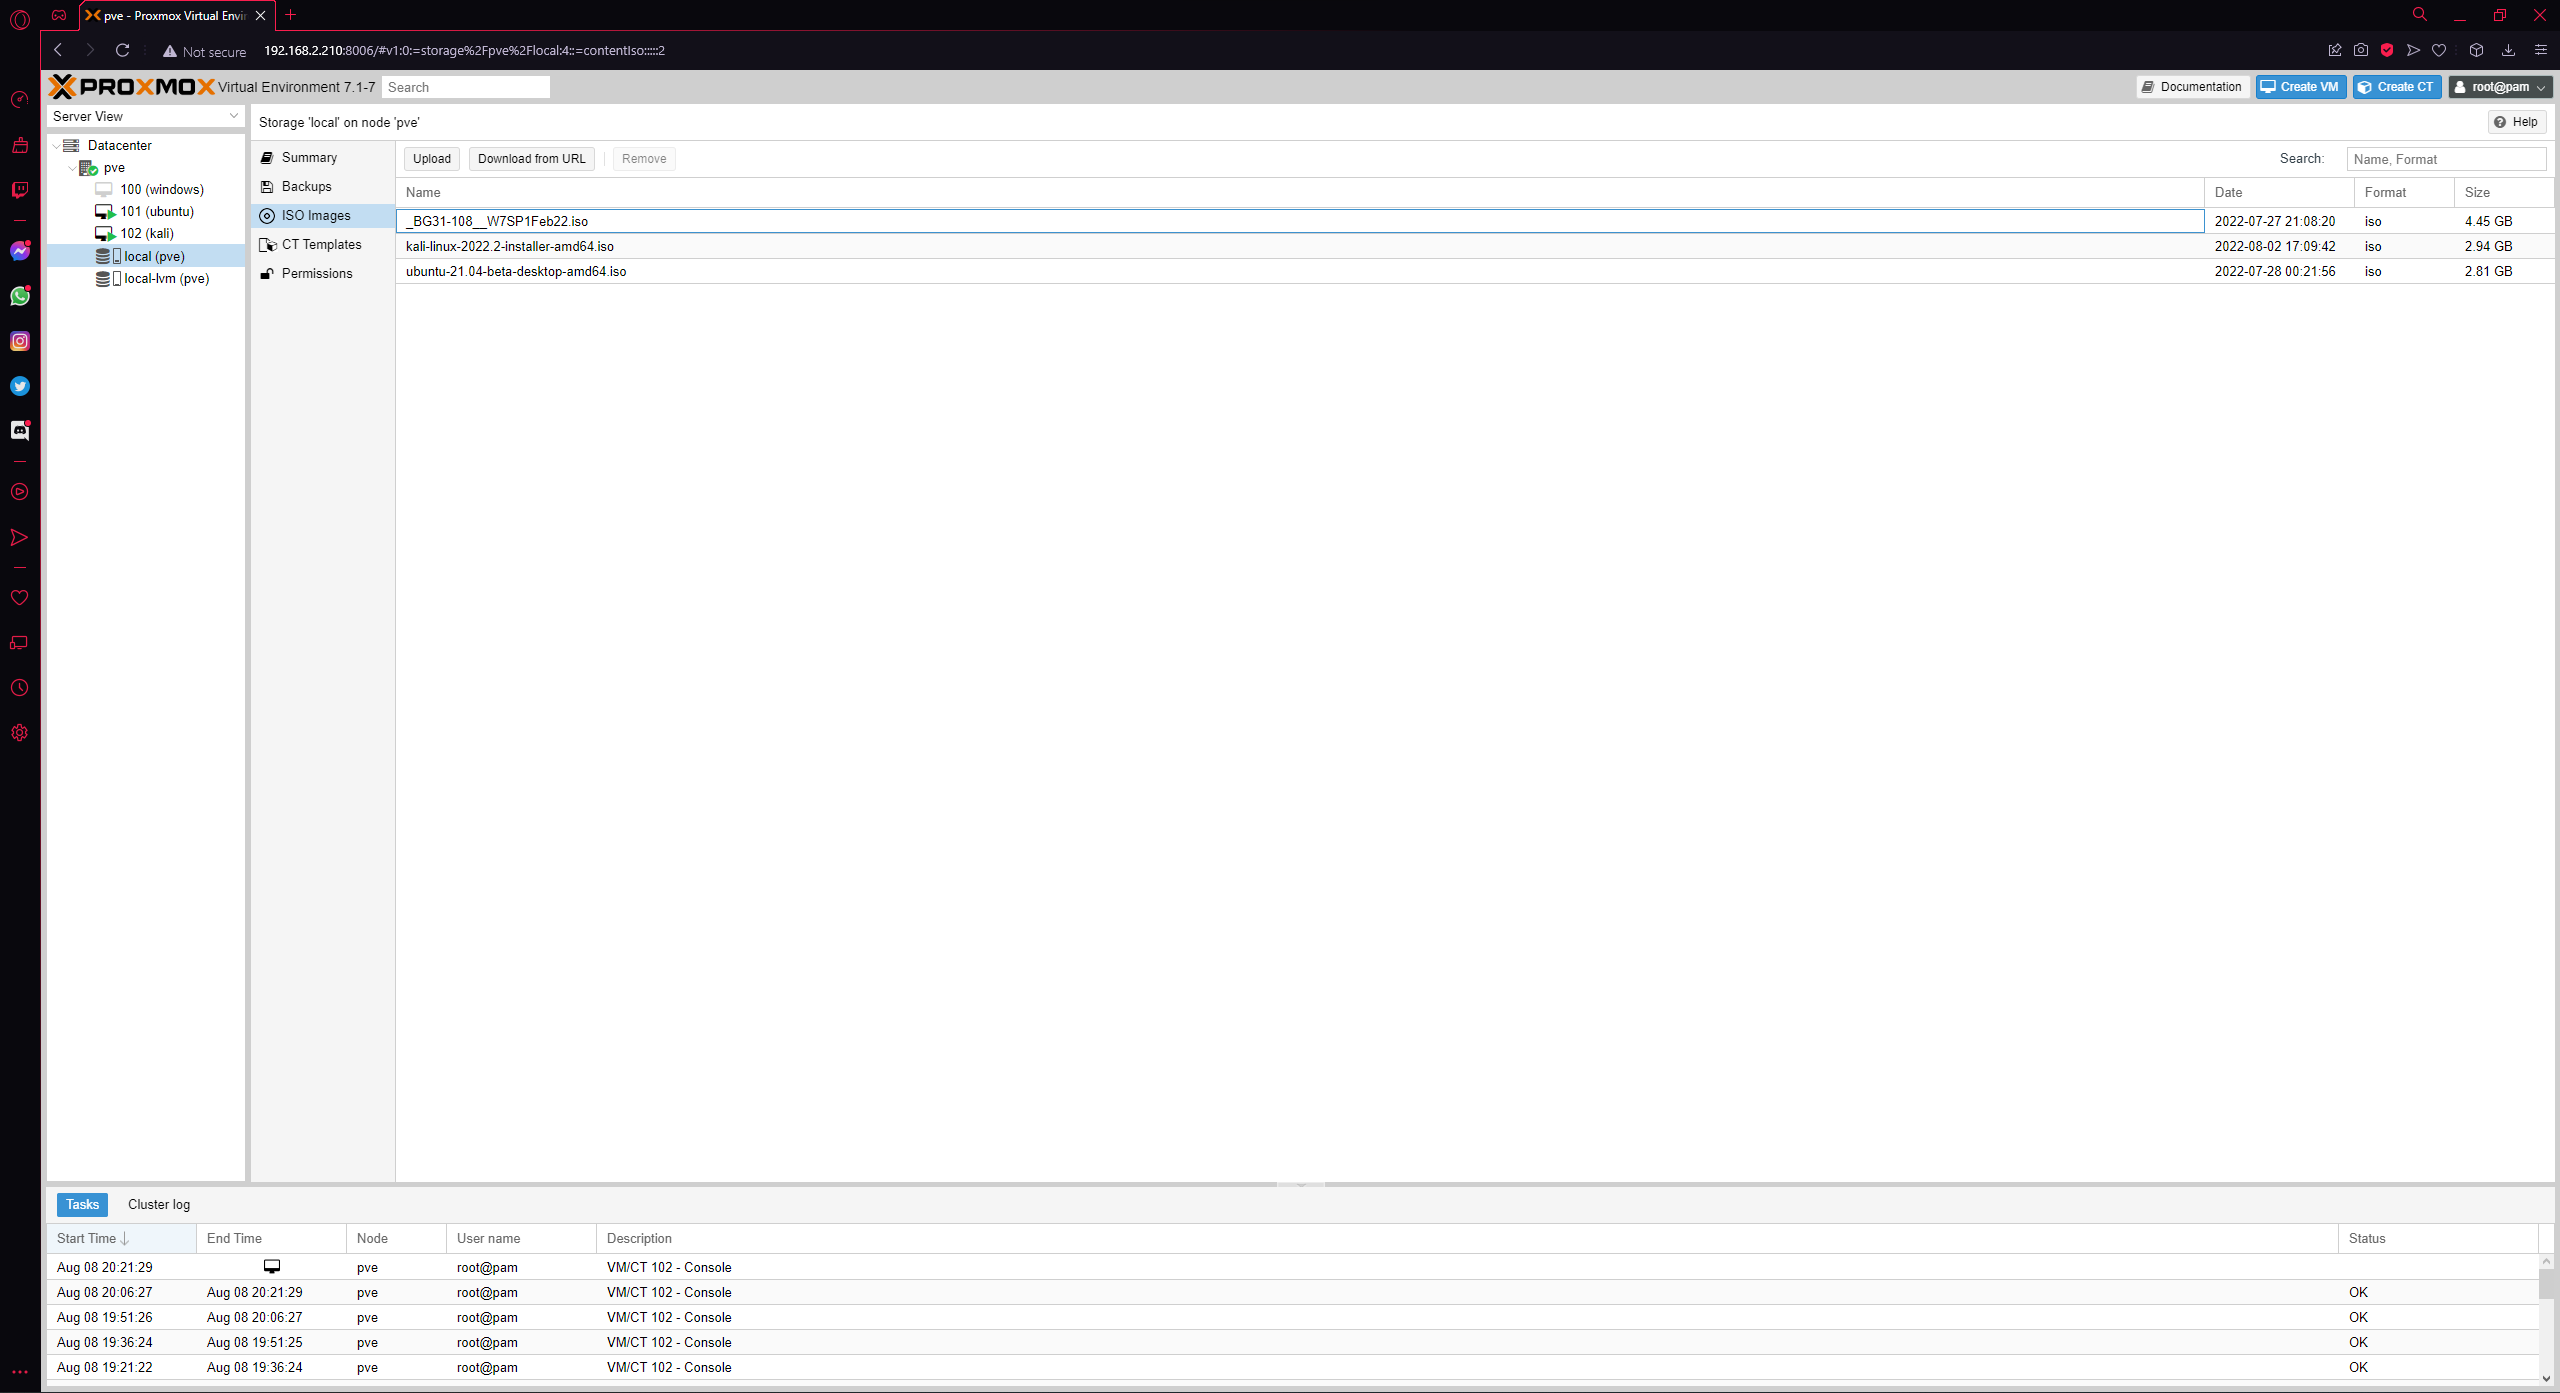
\includegraphics[width=0.7\linewidth]{upload iso 1.png}
    \caption{Local (PVE)}
  \end{figure}
  \newpage

  Pada menu ISO Images, klik upload, maka akan muncul tampilan seperti berikut. Setelah itu Select File pada ISO yang akan diupload lalu pilih upload.
  \begin{figure}[h!]
    \centering
    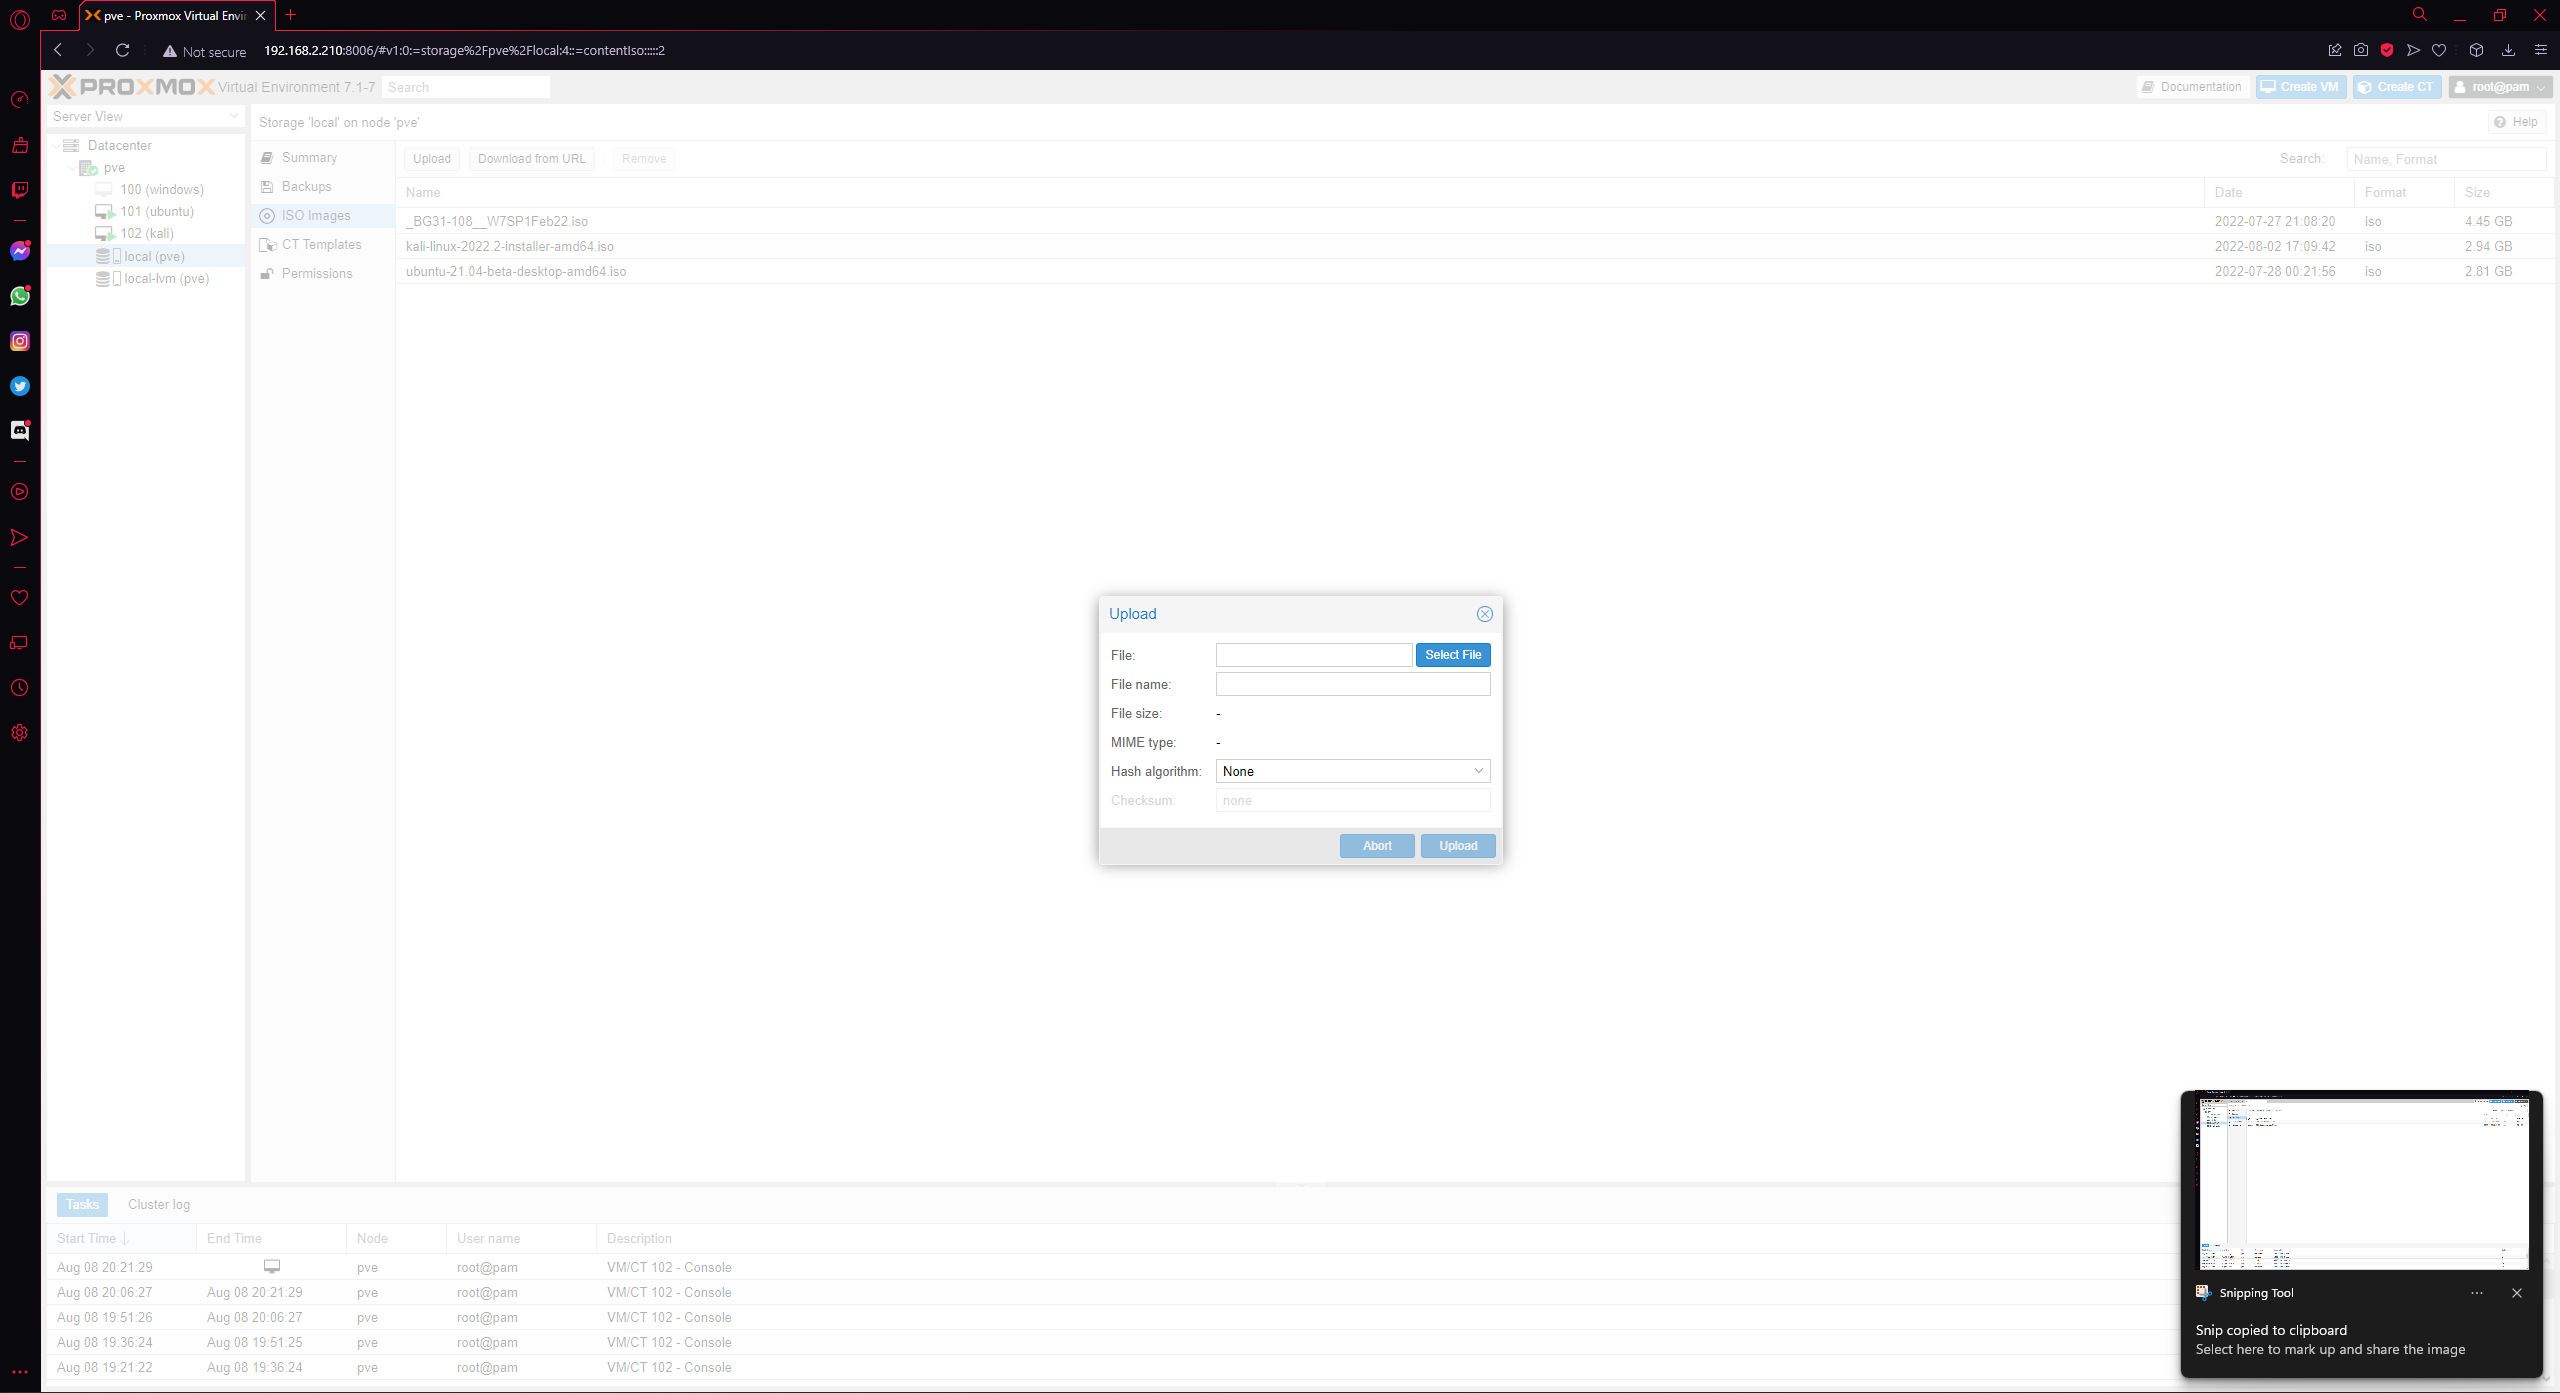
\includegraphics[width=0.7\linewidth]{upload iso 2.png}
    \caption{Upload ISO Image 1}
  \end{figure}

  Setelah upload ISO maka tampilan akan seperti berikut. Setelah itu tekan tombol Upload
  \begin{figure}[h!]
    \centering
    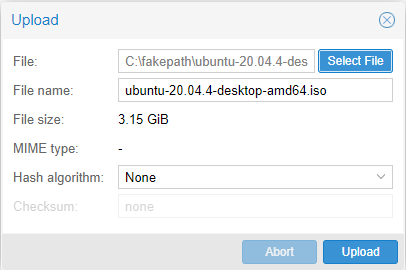
\includegraphics[width=0.7\linewidth]{upload iso 3.png}
    \caption{Upload ISO Image 2}
  \end{figure}
  \newpage
  
  Berikut merupakan tampilan jika telah mengupload ISO. Tekan tombol x untuk keluar.
  \begin{figure}[h!]
    \centering
    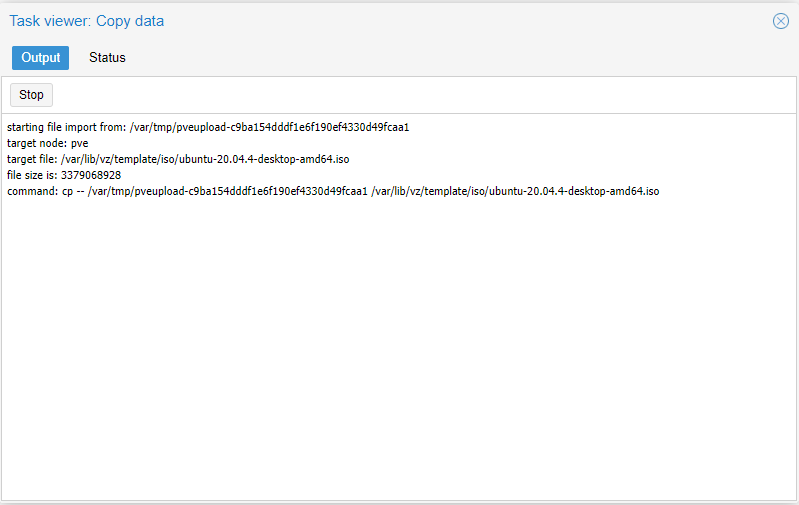
\includegraphics[width=0.7\linewidth]{upload iso 4.png}
    \caption{Upload ISO Image 3}
  \end{figure}
  \newpage

  \subsection{Membuat VM}
  Setelah selesai mengupload ISO, proses yang akan dilakukan selanjutnya adalah membuat VM.
  \begin{enumerate}
  \item Untuk membuat VM hal yang dilakukan adalah klik kanan pada node pve lalu tekan Create VM.
  \begin{figure}[h!]
    \centering
    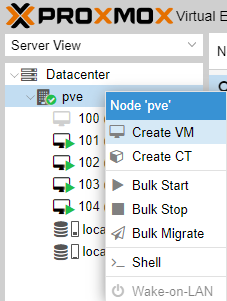
\includegraphics[width=0.7\linewidth]{create vm 1 a.png}
    \caption{Membuat VM a}
  \end{figure}
  \\ Atau klik Create VM pada menu diatas kanan Web GUI.
  \begin{figure}[h!]
    \centering
    
\includegraphics[width=0.7\linewidth]{create vm 1 b.png}
    \caption{Membuat VM b}
  \end{figure}
  \newpage
  \item Masukkan nama VM lalu tekan Next.
  \begin{figure}[h!]
    \centering
    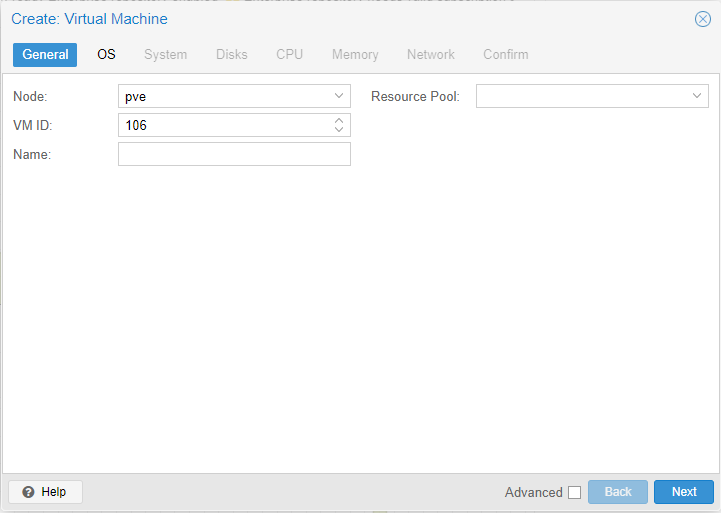
\includegraphics[width=0.7\linewidth]{create vm 2 a.png}
    \caption{Membuat VM a}
  \end{figure}
  \begin{figure}[h!]
    \centering
    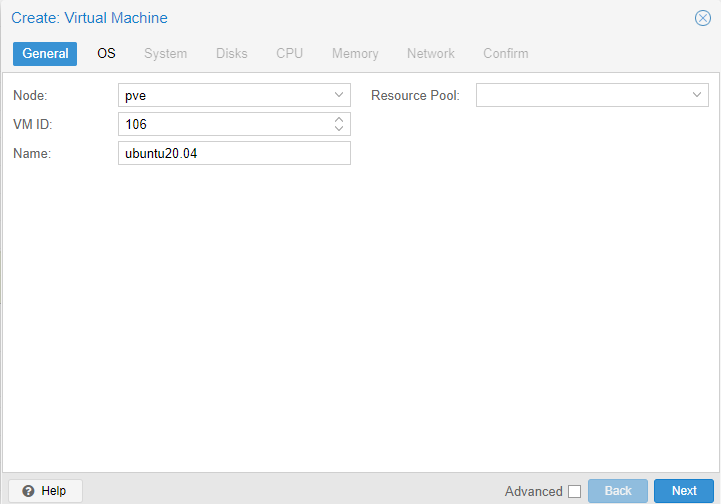
\includegraphics[width=0.7\linewidth]{create vm 2 b.png}
    \caption{Membuat VM b}
  \end{figure}
  \newpage
  \item Pilih ISO Image yang akan digunakan pada VM, setelah itu tekan Next.
  \begin{figure}[h!]
    \centering
    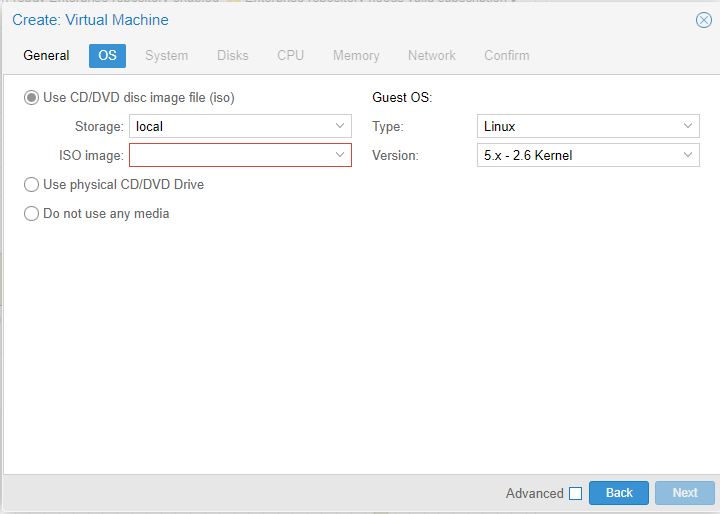
\includegraphics[width=0.7\linewidth]{create vm 3 a.png}
    \caption{Membuat VM a}
  \end{figure}
  \begin{figure}[h!]
    \centering
    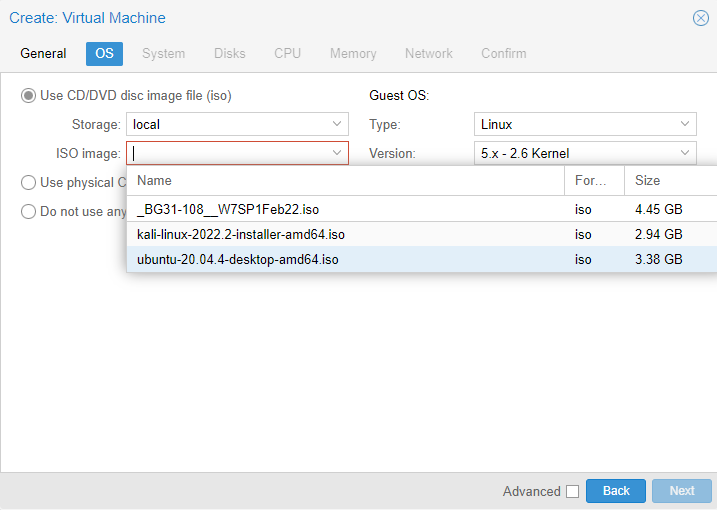
\includegraphics[width=0.7\linewidth]{create vm 3 b.png}
    \caption{Membuat VM b}
  \end{figure}
  \begin{figure}[h!]
    \centering
    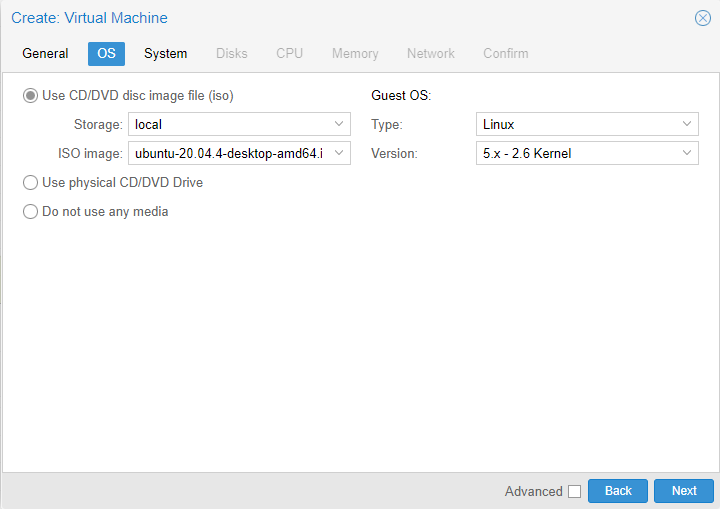
\includegraphics[width=0.7\linewidth]{create vm 3 c.png}
    \caption{Membuat VM c}
  \end{figure}
  \end{enumerate}

\end{document}